\chapter{基于代码审查图的代码结构可视化和质量分析}
\section{引言}

变更影响分析的结果能在一定程度上反映代码的质量,尤其是在代码的可维护性方面。对于一个方法,与其存在变更影响关系的方法越多,则说明该方法与其他方法耦合过深,难以维护。但是现有的方法并未将变更影响关系的分析结果与代码质量相结合,导致其在衡量代码可维护性方面的应用受限。此外,方法间的变更影响关系具有涟漪效应,体现了项目代码在宏观层面的结构关联性。开发者在维护代码时,需要明确变更影响的传播范围与路径,以评估潜在风险并制定合理的修改方案。然而,当前缺乏能够从宏观视角直观展示影响扩散情况的方法,开发者仍主要依赖人工阅读代码来理解系统依赖,这种方式效率低下,难以适应大规模软件系统的演化需求。

不局限在变更影响分析的过程中,在软件开发过程中的多个阶段,项目参与者都需要对项目代码结构有足够的了解。在初期阶段,开发者需要阅读和理解代码,对于大型项目,这一过程通常非常耗时。除此之外,开发者在代码变更时,如添加新功能或修复缺陷,需要深入了解对应代码的上下文信息。如果对上下文理解不清晰,可能会导致变更不完全或不准确,进而影响软件质量。在开发后期,开发者往往需要作为审查者参与到代码审查过程中。代码审查的主要目的是评估变更后代码是否符合质量标准,是否能合入主分支。这一过程在协作开发中至关重要,也是确保软件质量的有效手段。代码审查往往需要投入大量的时间和精力\cite{花子涵2024代码审查自动化研究综述},审查者不仅需要分析变更代码本身,还需要理解这些代码所处的上下文才能准确判断。因此,无论是开发者还是审查者,理解软件项目的代码结构都至关重要。只有深入掌握软件的整体架构和各模块之间的关系,才能在开发和审查过程中保证代码质量。因此,面对庞大复杂的代码库,如何在减少时间和精力消耗的同时,提高代码阅读和理解的效率与准确性,仍是一个重要挑战。

为了帮助开发者提高理解项目代码结构的效率并有效结合变更影响分析的结果,本文提出了代码审查图的概念,并基于代码审查图进行代码结构可视化和质量分析。通过将项目中的各个方法和全局变量表示为图的节点,用边表示方法与方法之间、方法与全局变量之间的依赖关系、耦合关系和变更影响关系,从而形成一个结构化的代码关系图。这样的图形化展示方式能够帮助开发者和审查者从宏观的角度掌握整个软件项目的架构和各个模块之间的关系,进而提升对代码的理解效率。通过这种方式,开发者和审查者可以更直观地识别出项目中的关键部分及其相互依赖关系,从而在变更和审查过程中更高效地评估代码的质量和影响。

\section{基于代码度量的代码质量度量模型}

结合变更影响分析的结果,并在此基础上对代码质量度量进行扩展,在代码结构的角度上衡量代码质量,本节提出基于代码度量的代码质量度量模型,度量结果作为代码审查图的节点属性的一部分,在可视化部分中进行展示。接下来详细介绍代码质量度量模型。

\subsection{代码质量度量模型}
\label{3_代码质量度量模型}


代码质量度量模型用于评估和量化软件代码质量,本文研究对象是方法以及模块的代码质量,参考Huang等人的工作\cite{黄沛杰2011代码质量静态度量的研究与应用},本文选取具有代表性的以下5个方面的质量属性和对应的18个度量元来进行衡量。

\begin{figure}[h]
\centering
\includegraphics[width = 1.0\textwidth]{figures/3_度量模型.pdf}
\caption{代码质量度量模型}
\end{figure}

一般而言,代码质量评价可分为绝对评价和相对评价两种。对于具有相同设计目的的一组代码,相对评价更具适用性\cite{黄沛杰2011代码质量静态度量的研究与应用}。在一个软件项目中,各个模块或方法通常具有相似的设计目标,因此,使用相对评价有助于开发者关注到项目代码中相对来说质量较差的代码,从而优化项目整体质量。

\paragraph{度量元度量} 对于度量值越小越好的度量元,假设代码$c$的质量属性$k$中子属性$i$度量元$j$对应的最大值和最小值分别是$\max_{ij}$和$\min_{ij}$,测试值区间 \(Z_{ij}\) 和测试值 \(t_{ij}\) 在 \(Z_{ij}\) 中的位置 \(t'_{ij}\) 分别为:
\begin{align}
Z_{ij} = \max_{ij} - \min_{ij}
\end{align}
\begin{align}
t'_{ij} = t_{ij} - \min_{ij}
\end{align}

使用统计中常用的分档方式,分五个档次对应优、良、中、差、极差,按式\ref{4_分档}的方式给定参考分值。
\begin{align}
\label{4_分档}
V_{ij}^c = 
\begin{cases} 
100, & t'_{ij} \leq 0.2Z_{ij} \\ 
80, & 0.2Z_{ij} < t'_{ij} \leq 0.4Z_{ij} \\ 
60, & 0.4Z_{ij} < t'_{ij} \leq 0.6Z_{ij} \\ 
40, & 0.6Z_{ij} < t'_{ij} \leq 0.8Z_{ij} \\ 
20, & 0.8Z_{ij} < t'_{ij}
\end{cases}
\end{align}

对于度量值越大越好的度量元,只需把式中分值倒序。

\paragraph{质量子属性度量} 一个质量子属性包含一个或多个度量元,将一个子属性下的所有度量元进行组合,总的评估质量子属性。定义代码c的子属性度量$U_{i}^c$ 如式\ref{4_质量子属性},这里将各度量元的权重设为等值。

\begin{align}
\label{4_质量子属性}
U_i^c = \sum_j w_{ij} V_{ij}^c, \quad \sum_j w_{ij} = 1
\end{align}

\paragraph{质量属性度量} 对质量属性下的子属性进一步计算得到代码质量属性度量,计算公式如式\ref{4_质量属性总计},这里将各子属性的权重设为等值。

\begin{align}
\label{4_质量属性总计}
Q_k^c = \sum_i w_{ki} U_{i}^c, \quad \sum_i w_{ki} = 1
\end{align}

质量属性度量作为代码在某一方面的质量表现情况,在实际情况下可单独使用,因此这里不再对质量属性度量进一步聚合评分。除此之外,每一层级的质量属性均可如式\ref{4_分档}所示对度量进行相对分档,以评价相对质量表现情况。

\subsection{基于内聚度缺乏度和连通性的的内聚性度量}

\noindent \textbf{1.基于内聚度缺乏度的内聚度计算}

 LCOM(Lack of Cohesion in Methods)系列指标是根据模块内聚度的缺乏程度来衡量模块的内聚度的指标。在本文中,
面向对象语言以类为研究范围进行计算内聚度,非面向对象的语言以文件为研究范围进行计算,类中的成员属性对应文件中的全局变量,类中的成员方法对应文件中定义的方法。LCOM 指标的核心思想是度量一个类中方法
对实例变量(属性)的共享程度。不同版本的 LCOM 有着不同的计算方法和含义,体现了不同的侧重点。本文共计算以下四个指标。

(1)LCOM1,含义是不引用相同字段的方法对数目\cite{1994Ametr}。计算公式如式\ref{4_LCOM1}。
\begin{equation}
\label{4_LCOM1}
LCOM1 = C_{n}^{2}-e
\end{equation}

其中n 是文件中的方法总数,e 是引用相同字段的方法对。以图\ref{4_示例模块}为例介绍计算过程,其中椭圆表示方法,点表示变量,点在椭圆内表示该方法引用了该变量。如图所示模块的LCOM1值为\(C_{6}^{2} - 5 = 10\)。

\begin{figure}[h]
\centering
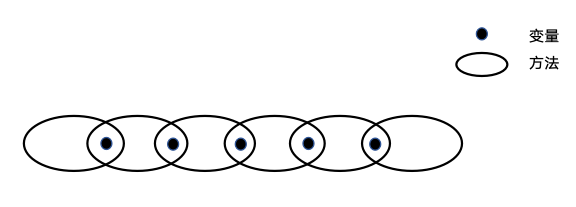
\includegraphics[width = 0.7\textwidth]{内聚度示例.jpg}
\caption{示例模块}
\label{4_示例模块}
\end{figure}
    

(2)LCOM2,含义是不引用相同字段方法对与引用相同字段方法对数之差\cite{1996Coupling}。其计算公式如式\ref{4_LCOM2}。

\begin{equation}
\label{4_LCOM2}
    {LCOM2}=\left\{
        \begin{array}
        {c}P-Q,  ifP\geq Q \\
        0,  otherwise
        \end{array}\right.
\end{equation}

其中,P 是不共享实例变量的方法对的数量,Q 是共享实例变量的方法对的数量。
如果 LCOM2 的结果为负数,则被置为 0。图\ref{4_示例模块}模块中,不共享变量的方法对P为10,共享变量的方法对Q为5,LCOM2值为P-Q=5。

(3)LCOM3是对前两种指标的进一步改进,其计算公式如式\ref{4_LCOM3}:
\begin{equation}
\label{4_LCOM3}
LCOM3 = \frac{\left( \frac{1}{a} \sum_{j=1}^a \mu(A_j) \right) - m}{1 - m}
\end{equation}

其中\( m\)为文件中的方法数,\( a\)表示文件中的变量数,\( mu(A_j)\)表示的是引用变量\(A_j\)的方法数。如图\ref{4_LCOM3计算示例}所示的文件中有3个方法和3个变量,计算过程如图所示。
\begin{figure}[h]
\centering
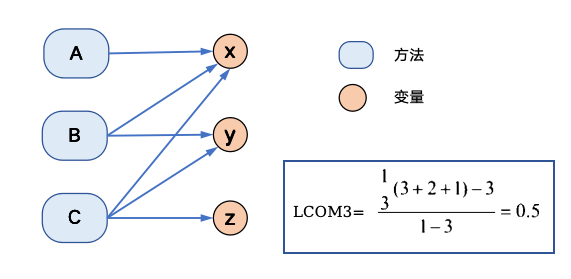
\includegraphics[width = 0.7\textwidth]{LCOM3.jpg}
\caption{LCOM3计算示例}
\label{4_LCOM3计算示例}
\end{figure}



(4)LCOM4,含义是以方法和变量为顶点,方法引用字段或方法之间有调用关系则两节点之间有条边构成图的连通分支数\cite{1995Measuring}。计算时,根据深度优先搜索的方式,计算图中的连通分支数,得到的值即为LCOM4。如图\ref{4_LCOM4计算示例}所示的两个文件的LCOM4的值分别为2和1。

\begin{figure}[h]
\centering
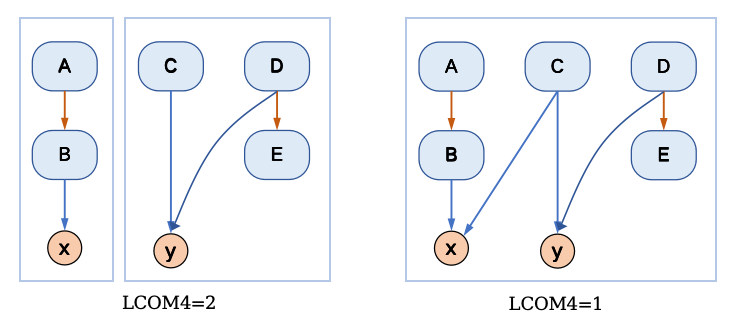
\includegraphics[width = 0.7\textwidth]{LCOM4.jpg}
\caption{LCOM4计算示例}
\label{4_LCOM4计算示例}
\end{figure}

\noindent \textbf{2.基于连通性的内聚度计算}

TCC(Tight Class Cohesion)和 LCC(Loose Class Cohesion)是用于衡量模块内
聚度的指标,这两个指标主要关注于模块中方法之间的连通关系,核心思想是通过
分析模块中方法如何相互作用以及如何访问共同资源(如全局变量)来评估模块的内聚度。

(1)TCC,含义是有连通关系的方法对数与总方法对数的比值\cite{1995Cohesion}。
TCC 关注于模块中方法之间的“直接连接”。如果两个方法直接共享访问同一个变
量,则认为这两个方法是直接连接的。计算公式如式\ref{4_TCC}。
\begin{equation}
\label{4_TCC}
{TCC} = \frac{e}{C_{n}^{2}}
\end{equation}

其中\(n\)是文件中的方法总数,\(e\)是图中的直接连接边数。

(2)LCC则基于方法间接引用共同字段的关系进行计算\cite{1995Cohesion}。
LCC 除了考虑直接连接的方法对外,还包括了间接连接的方法对。如果两个方法不
是直接连接,但可以通过一系列的方法调用或变量引用来连接,则认为它们是间接连接的。LCC 的值基于模块中直接或间接连接的方法对占所有可能方法对的比例来计算。因此,LCC 的值通常不低于 TCC 的值,提供了一个更宽泛的模块内聚度视角。计算公式如式\ref{4_LCC}:
\begin{equation}
\label{4_LCC}
{LCC=\frac{e+e_{indirect}}{C_{n}^{2}}}
\end{equation}

其中\(n\)是文件中的方法总数,\(e\)是图中的直接连接边,\(e_{indirect}\)是除直接连接边的边数。如图\ref{4_TCC和LCC计算示例}是计算LCC和TCC的例子,左图中通过方法AB通过变量x直接连接,方法CD通过变量y直接连接,直接连接和间接连接都是2。而右图中直接连接是AB、BC、BC和CD,间接连接是AD和BD,计算结果如图所示。

\begin{figure}[h]
\centering
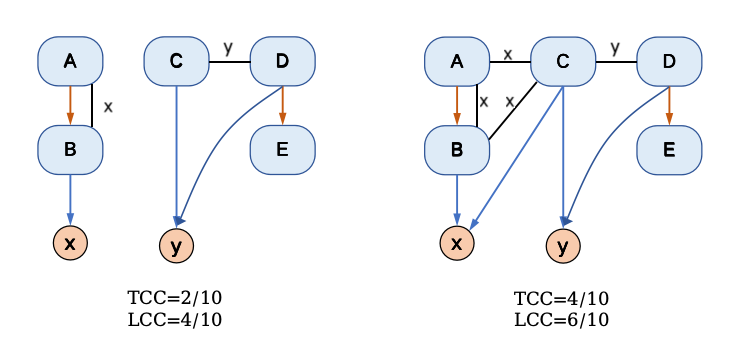
\includegraphics[width = 0.7\textwidth]{TCCLCC.jpg}
\caption{TCC和LCC计算示例}
\label{4_TCC和LCC计算示例}
\end{figure}


\subsection{方法间耦合性度量}

耦合性是在软件架构中用来描述模块间相互依赖和连接程度的一个重要指标。耦合度的高低会影响系统的可维护性和可复用性。在现有的研究和实践中,耦合度通常被细分为六个等级\cite{DNZS200722064},如表\ref{4_软件架构中耦合性分类}所示,这些等级从高到低反映了模块间依赖的紧密程度。本文关注的是方法与方法之间的耦合性。通过深入分析方法间的耦合,反映方法如何通过参数传递、调用关系、共享全局变量等方式相互依赖,可以更准确地识别潜在的设计缺陷和优化机会,从而提高系统的模块化程度,增强系统的可维护性和可扩展性。

\begin{table}[htbp]
\caption{软件架构中耦合性分类}
\label{4_软件架构中耦合性分类}
\vspace{0.5em}\centering\wuhao
\begin{tabular}{ccccc}
\toprule
耦合性类别 & 描述 & 耦合程度 & 本文是否分析 \\
\midrule
内容耦合 & 模块直接访问或修改另一个模块的内部数据 & 6 & 否\\
公共耦合 & 模块访问同一公共数据环境 & 5 & 是 \\
外部耦合 & 模块共享全局简单数据结构 & 4 & 是 \\
控制耦合 & 模块传递控制信息,影响计算流程 & 3 & 否 \\
标记耦合 & 通过参数传递复杂数据结构信息 & 2 & 是 \\
数据耦合 & 通过参数传递简单数据 & 1 & 是 \\
\bottomrule
\end{tabular}
\end{table}

接下来详细介绍这几种耦合的含义和计算方式。(1)内容耦合是耦合度最高的一种形式,表示一个模块能够直接访问或修改另一个模块的内部数据和结构。在方法级的耦合分析中,这种耦合形式通常不被考虑,因为方法间的直接数据访问往往通过参数传递或者 API 调用实现,而不是直接的内容访问。(2)公共耦合发生在多个模块共同访问某个全局数据环境时。这种数据环境可能是全局数据结构、全局变量或内存公共区域等。在提取到的全局变量表中,对于复杂数据结构如结构体和数组,其引用点所在的方法之间均存在公共耦合关系。(3)外部耦合与公共耦合相似,但区别在于它涉及的是对全局简单变量的访问。例如,当多个模块访问或修改相同的全局简单类型变量时,则这些模块之间存在外部耦合。(4)控制耦合指模块之间传递信息中包含用于控制模块内部的信息。由于本文不考虑分析方法内部逻辑,因此不提取此种耦合。(5)标记耦合指通过参数表传递数据结构信息,调用时传递的是数据结构。在方法摘要表中检查方法的参数信息,根据参数类型,可确定参数表中是否包含复杂类型。除此之外,在方法的调用表中,也提取了方法调用的其他方法,结合这两个信息,即可确定两个方法是否存在着标记耦合关系。(6)数据耦合指通过参数表传递简单数据。与标记耦合类似,根据参数类型可以确定参数是否全部为基本类型,结合方法调用表,即可确定两个方法是否存在数据耦合。

\subsection{方法扇入扇出度量}

方法的扇入(Fan-in)和扇出(Fan-out)是软件工程中常用于衡量方法可复用性和方法复杂性的两个指标。



扇入是指调用某个方法的不同方法的数量。扇入值较高的方法通常被认为是重要的或核心的,因为它们被多个其他方法所依赖。高扇入值可能意味着该方法执行了一个基础或共享的任务。可复用性较强。

扇出指的是一个方法直接调用的其他方法的数量,反映了该方法对外部方法的依赖程度。较高的扇出值通常意味着该方法需要管理和协调更多的外部操作。在软件工程中,较高的扇出值可能导致方法的责任范围过大,进而影响代码的可复用性,较高的扇出可能使得该方法难以在不同的上下文中独立使用或重用。因此,扇出值较高的代码常常提示着潜在的复杂性问题,可能需要进行分解和增加中间层方法的方式进行重构,如图\ref{4_高扇出及其分解示例}所示,以减少对外部方法的依赖,提升其可复用性和灵活性。

\begin{figure}[h]
\centering
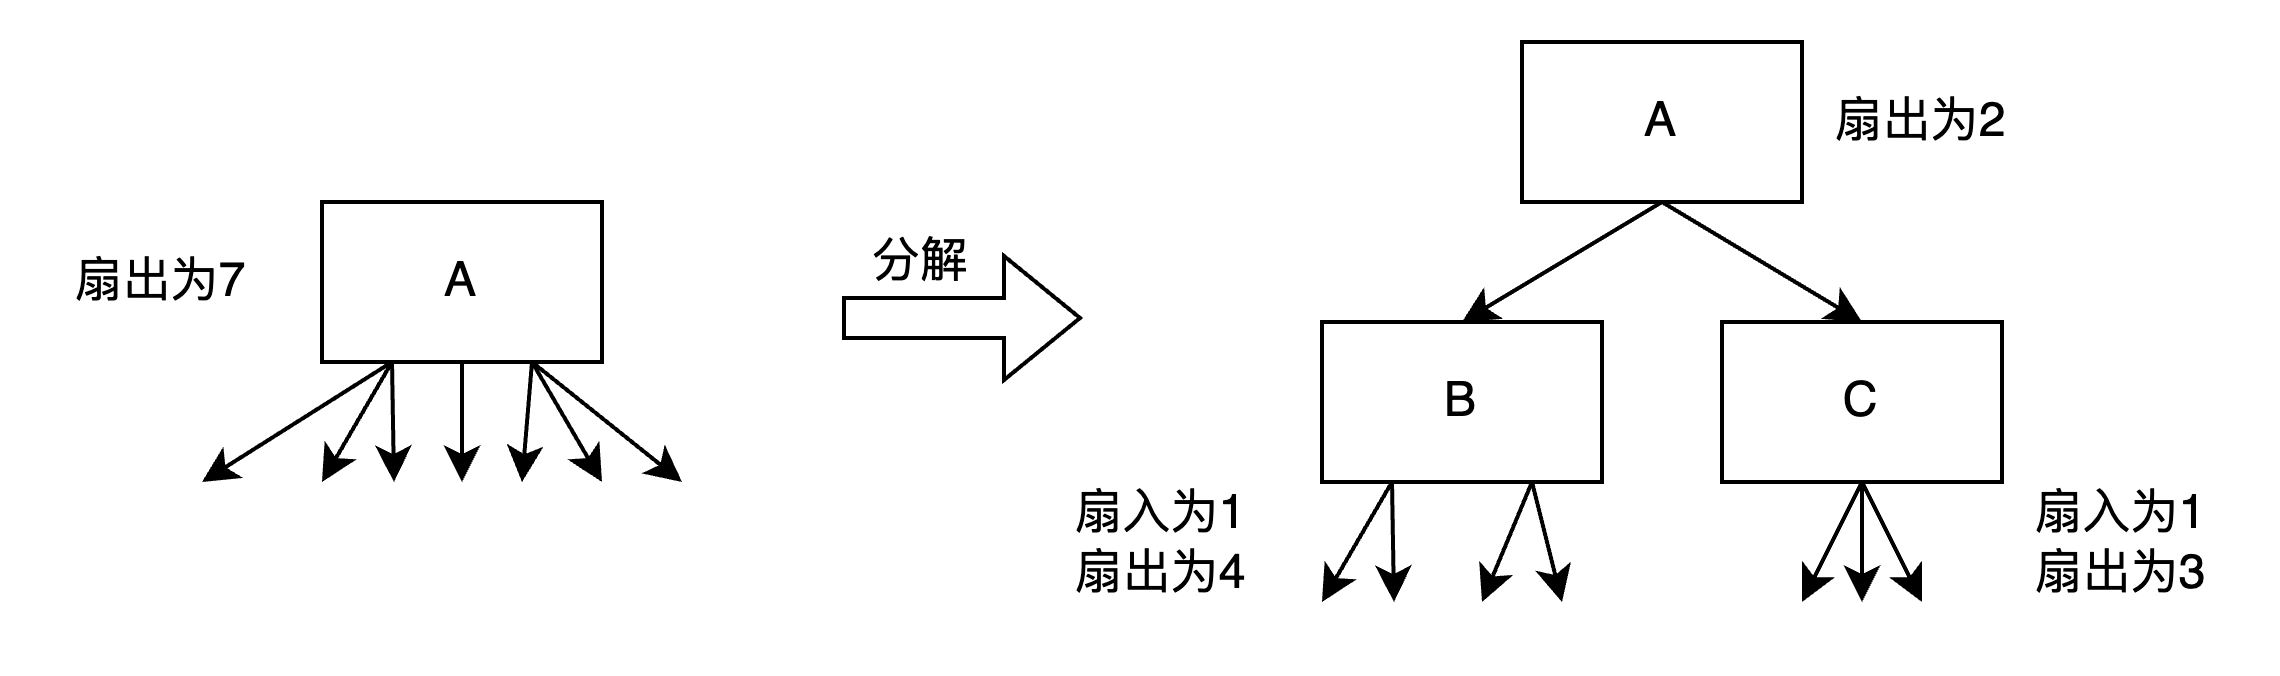
\includegraphics[width = 0.8\textwidth]{figures/扇出介绍.jpg}
\caption{高扇出及其分解示例}
\label{4_高扇出及其分解示例}
\end{figure}

本文中对于提取到的方法摘要表,遍历每一个方法,统计其调用方法的数量即可计算出该方法的扇出值,再以该方法名在方法摘要表中搜索调用了该方法的方法,统计总数,得到的值即为扇入值。

\subsection{基于静态检测工具的代码度量}

在安全性和规范性代码属性中,使用静态代码分析工具 Cppcheck对项目中的源代码进行检测和分析。Cppcheck 是一款开源的静态分析工具\footnote{http://cppcheck.net/},专门用于检测 C/C++ 代码中的缺陷、潜在错误和编码规范问题。Cppcheck会根据问题的严重性和类别将检测出的问题如表\ref{4_cppcheck报告问题分类}所示的六类。

\begin{table}[htbp]
\caption{cppcheck报告问题分类}
\label{4_cppcheck报告问题分类}
\vspace{0.5em}\centering\wuhao
\begin{tabular}{cp{12cm}}
\toprule
类别 & 描述 \\
\midrule
error & 严重错误,通常包括内存泄漏、缓冲区溢出、空指针解引用等致命问题 \\
warning & 潜在的错误或不推荐的做法,如不安全的类型转换等 \\
style & 代码风格问题,通常与代码格式、命名约定等相关,例如变量命名不规范等 \\
performance & 性能问题,表明当前方式可能效率不高,例如重复计算、低效循环等 \\
portability & 平台相关问题,可能导致在不同环境出现不同行为,例如操作系统特有的API调用、字节序问题等 \\
information & 额外的信息或建议,例如推荐的编码实践等 \\
\bottomrule
\end{tabular}
\end{table}


检测结果中包括了诸如错误、警告和代码风格问题等不同级别的信息,这些信息帮助开发者识别代码中的潜在问题。我们将前两类作为安全性度量元,将style和performance类别的问题数作为规范性度量元进行计算。portability和information由于并不是代码本身的质量问题,因此不进行计算。

在复杂性属性中,使用lizard提取方法的圈复杂度,它是一个轻量级的源代码复杂度分析工具\footnote{https://github.com/terryyin/lizard},可以按方法或文件等不同的粒度计算圈复杂度,这里我们分析对象为方法级。

静态工具提供的报告与其他度量指标相结合,共同构成了全面的质量评估体系。通过这种方式,本研究实现了对代码质量的多维度综合评价,为开发者提供了更为直观的质量评估和改进方向。

\section{代码审查图的构建和可视化}

在软件开发过程中,开发者通常需要从全局的角度了解项目的结构以及模块之间的关系。然而,随着项目规模的扩大,代码的复杂性也会急剧增加,这使得传统方式难以有效地展示全局视图。因此,为了更好地帮助开发者在复杂的项目中进行有效的代码审查和质量评估、以及更安全地维护变更,本章提出代码审查图的概念,介绍其构建和可视化过程,以帮助从直观的角度理解项目代码结构,掌握代码质量。

\subsection{代码审查图构建}

代码审查图由两个核心元素构成,分别是节点和边。其中,节点代表软件项目代码的关键元素,包括方法和全局变量。边表示节点之间的关系,包括耦合关系、变更影响关系以及依赖调用关系。接下来详细介绍节点和边的构成。

\noindent \textbf{1.节点设计}

节点用于标识项目中的方法和全局变量。根据前文方法提取到的方法摘要表和全局变量信息表,为每个方法和全局变量创建对应的节点。每个节点具有多种属性,提供有关节点所代表的方法或变量的关键信息,便于开发者对代码进行全面的审查和分析。

方法属性分为两个主要部分:首先是方法的基本信息,如表\ref{4_代码审查图节点属性-基本信息}所示。

\begin{table}[htbp]
\caption{代码审查图节点属性-基本信息}
\label{4_代码审查图节点属性-基本信息}
\vspace{0.5em}\centering\wuhao
\begin{tabular}{cccc}
\toprule
    属性 & 描述 \\
\midrule
方法名 & 方法名,由方法所在路径和方法名拼接而成,保证唯一  \\
方法参数 & 方法的参数列表,包括参数的名称和类型   \\
方法内调用方法 & 本方法内调用的其他方法名   \\
方法可作用域 & 表明方法是否全局可用   \\
方法所在模块 &  方法所在模块,目前表示为方法所在文件  \\ 
\bottomrule
\end{tabular}
\end{table}

这一部分包括方法的名称、所在模块、方法签名、访问修饰符等,这些属性有助于开发者了解方法的基本信息。例如,方法的名称可以反映其业务功能,所在模块和作用域则有助于理解方法的上下文和调用约束等。

其次是与代码质量相关的度量和信息,如表\ref{4_代码审查图节点属性-质量相关信息}所示。

\begin{table}[htbp]
    \caption{代码审查图节点属性-质量相关信息}
    \label{4_代码审查图节点属性-质量相关信息}
    \vspace{0.5em}\centering\wuhao
    \begin{tabular}{cp{6cm}p{6cm}}
    \toprule
    质量子属性 & 度量元 & 描述 \\
    \midrule
    内聚性& LCOM1、LCOM2、LCOM3、LCOM4、TCC、LCC &  总的相对评分、相应建议、具体的属性值 \\           
    耦合性& 数据、标记、外部、公共耦合数 &  总的相对评分、建议、与本方法存在数据、标记、外部、公共耦合关系的方法 \\       
    变更影响 & 变更影响关系数 & 总的相对评分、与本方法存在变更影响的方法 \\
    扇出 &扇出值 &  总的相对评分、建议、方法的扇出值 \\
    扇入 &扇入值 &  总的相对评分、建议、方法的扇入值 \\ 
    代码缺陷 & 严重缺陷数和潜在缺陷数 &  总的相对评分、cppcheck检测得到的本方法缺陷信息 \\    
    代码规范 &  规范和一致性问题数、代码性能问题数 &  总的相对评分、cppcheck检测得到的本方法规范性信息 \\    
    圈复杂度 & 圈复杂度 & 总的相对评分、圈复杂度\\    
    \bottomrule
    \end{tabular}
    \end{table}

这一部分将展示前文根据质量度量模型得到的代码的5种质量属性情况,包括可维护性、复杂性、可复用性、安全性和规范性五个方面,并且将这五个方面的特性根据度量进行分档,给出分档等级。同时为了进一步指导用户对具体质量子属性进行优化,还报告了质量子属性的相对质量情况,对于较差的子属性向开发者提供有针对性的改进建议。例如,如果某个方法的扇出度较差,则可能表明该方法在项目中的依赖关系过于复杂,可能需要拆分。类似地,如果某模块的内聚性较差,则说明模块内部各元素的依赖关系较为松散,指导用户对该模块进行重构。

\begin{table}[htbp]
\caption{代码审查图节点属性-全局变量信息}
\label{4_代码审查图节点属性-全局变量信息}
\vspace{0.5em}\centering\wuhao
\begin{tabular}{cccc}
\toprule
    属性 & 描述 \\
\midrule
变量名 & 全局变量名,由所在路径和变量名拼接而成,保证唯一  \\
变量类型 & 变量类型   \\
被使用方法 & 使用了本全局变量的方法名   \\
变量可使用域 & 表明变量是否全局可用   \\
方法所在模块 &  变量所在模块,目前表示为所在文件  \\  
\bottomrule
\end{tabular}
\end{table}

对于全局变量的属性则主要包含表\ref{4_代码审查图节点属性-全局变量信息}中的信息。主要是对全局变量基本信息的展示,方便开发者快速了解该变量的作用域、使用情况以及被引用情况。通过这些信息,开发者能够更好地理解变量在整个项目中的作用以及对应的代码上下文。



\noindent \textbf{2. 边的设计}

在代码审查图中,边表示节点与节点之间的关系,这些关系揭示了软件项目代码中方法与方法、方法与全局变量之间不同类型的联系。

根据边的性质,其类型主要分为三类,如表\ref{4_代码审查图边分类}所示,包括静态依赖关系、耦合关系和变更影响关系。其中静态依赖关系分包括方法之间的调用和方法对全局变量的引用,耦合关系如表中所示共4类,变更影响关系则由第三章方法检测得到。

\begin{table}[htbp]
\caption{代码审查图边分类}
\label{4_代码审查图边分类}
\vspace{0.5em}\centering\wuhao
\begin{tabular}{cccc}
\toprule
属性 & 描述 \\
\midrule
静态依赖关系 & 含方法之间调用、方法引用全局变量两种  \\
耦合关系 & 含数据耦合,标记耦合,外部耦合,公共耦合四种   \\
变更影响关系 & 由第三章方法检测得到  \\
\bottomrule
\end{tabular}
\end{table}

每种关系反映了不同类型的代码相互作用,揭示不同代码元素之间的联系,帮助开发者全面理解系统的代码结构。尤其是变更影响关系,辅助开发者在进行代码变更时了解变更的影响范围,防止不完全变更,保证代码质量。



\subsection{代码审查图可视化}

为将代码结构直观地展示给开发者,本节对前文构建的代码审查图进行可视化。接下来从代码审查图的可视化方案和交互方案两个方面展开介绍。

\noindent \textbf{1.可视化方案}


代码审查图的可视化方案基于开源项目 G6\footnote{https://github.com/antvis/g6}。G6 是一个强大的图形可视化引擎,提供了绘制、布局、分析、交互、动画等全方位的图形可视化基础功能,具有简单易用且完备的特性。G6 具有两个显著优势。

(1)数据与可视化图形分离:在使用 G6 时,用户只需将图的数据组织为 JSON 格式,如图\ref{4_G6图数据示例}所示,包括节点信息和边信息,直接传递给 G6 即可生成对应的力导向图。这种数据与图形分离的方式不仅简化了开发流程,还提高了数据的灵活性和可操作性,便于进行后续的数据更新和图形重绘。

\begin{figure}[h]
\centering
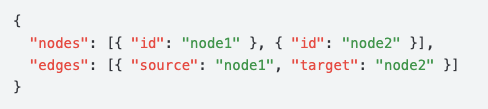
\includegraphics[width = 0.6\textwidth]{G6图数据示例.jpg}
\caption{G6图数据示例}
\label{4_G6图数据示例}
\end{figure}

(2)高度的定制能力:G6 提供了丰富的图形展示配置选项,用户可以根据需求自由选择不同的样式和布局方式。如果 G6 内置的元素不满足特定需求,它还支持用户自定义节点、边及其他元素,使得图形展示更加贴合实际应用场景。

本文使用G6内置节点和边实现代码审查图的可视化。G6的节点构成共包含6部分,其中label表示文本标签,通常用于展示节点的名称或描述,本文中将节点属性赋值给label,便于用户查看属性相关信息。G6的边的构成共包含4部分,label具有同样的功能,将边的类别用于label。让 G6 加载此数据源进行展示,就实现了同时也实现了计算逻辑与图形可视化的有效分离。

\noindent \textbf{2.交互方案}

在软件项目的代码分析中,方法和全局变量的数量往往达到数千级别。对于这样规模的图而言,难以在单个视图中完整展示所有信息。因此,需要通过用户交互机制,使开发者能够按需探索并查看更详细的代码关系与结构。表\ref{4_代码审查图交互和逻辑设计}展示了目前代码审查图的交互和对应的逻辑设计。


\begin{table}[htbp]
\caption{代码审查图交互和逻辑设计}
\label{4_代码审查图交互和逻辑设计}
\vspace{0.5em}\centering\wuhao
\begin{tabular}{cccc}
\toprule
交互方式 & 业务逻辑 \\
\midrule
视角缩放 & 操作鼠标滚轮对图进行缩放  \\
视角移动 & 鼠标拖拽移动整个代码审查图   \\
聚焦节点 & 光标悬停在节点上显示节点的方法名/变量名  \\
移动节点 & 鼠标长按节点拖拽可移动节点 \\
查看节点属性 & 鼠标点击节点展开节点属性  \\
聚焦关系 & 光标悬停在边上显示边的类型  \\
查看关系信息 & 鼠标点击节点展开节点属性  \\
节点筛选 & 通过点击筛选节点按钮,确认是否筛选掉孤立节点 \\
节点搜索 & 搜索模块、方法、全局变量名称,高亮对应节点 \\
\bottomrule
\end{tabular}
\end{table}


\section{基于代码审查图的代码质量分析}
\label{4_不良图模式}

代码审查图不仅能展示项目代码结构,还能直观地反映与代码质量相关的一些不良特征。通过对代码审查图的进一步分析,本文总结了6种不良的图模式。它们在不同的角度上反映了较差的代码结构,辅助开发者理解代码质量较差或较好的具体原因,并指明对应的优化方向。

\paragraph{1.冗余代码元素} 冗余代码元素指的是在代码中定义但从未被使用的代码元素。在代码审查图中表现为孤立节点,如图\ref{1_冗余代码图模式}所示。即某个节点不与任何其他节点存在边的图模式。这意味着该代码元素不和任何其他代码产生依赖、调用等联系,不论是作为全局变量还是方法出现,都会消耗不必要的性能和资源,且影响其所在模块的内聚程度。优化时,可以考虑去掉冗余代码,只保留和软件核心逻辑相关的代码。

\begin{figure}[h]
\centering
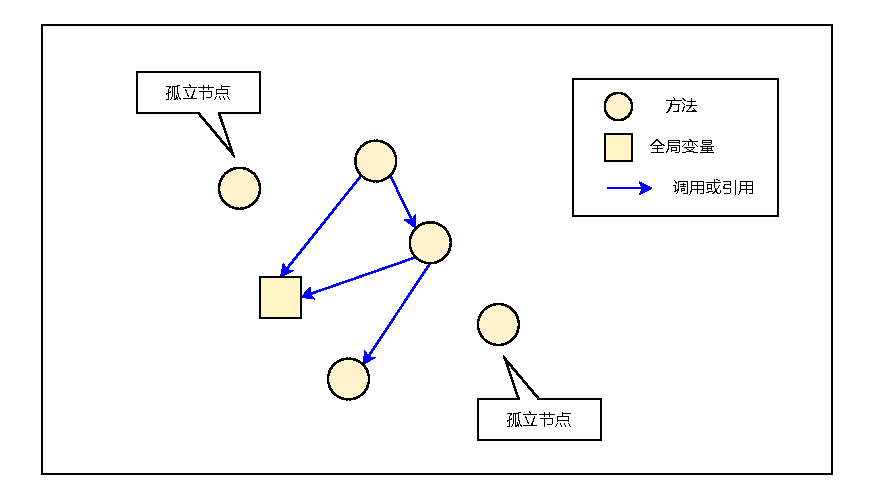
\includegraphics[width = 0.6\textwidth]{figures/孤立节点图模式_2.pdf}
\caption{冗余代码图模式}
\label{1_冗余代码图模式}
\end{figure}



\paragraph{2.长嵌套调用} 长嵌套调用在代码审查图中的表现方式是方法间的链式连接,如图\ref{1_长嵌套调用图模式}所示。长嵌套调用有以下几点危害,1.可读性差:层次过多的嵌套调用会使代码结构变得复杂,理解代码的执行顺序和逻辑变得困难。2.可维护性差:由于链式的松散结构,模块的可维护性也会变差,当需要对中间环节进行变更时,可能会影响整个嵌套调用的逻辑。3.性能问题:方法调用会涉及到栈帧的创建和销毁,长的嵌套调用会导致栈的深度增加,频繁的栈操作可能会影响性能。在代码审查图中可以直观地发现嵌套调用的现象。优化时可以考虑合并部分底层方法,减少嵌套层数来优化代码。

\begin{figure}[h]
\centering
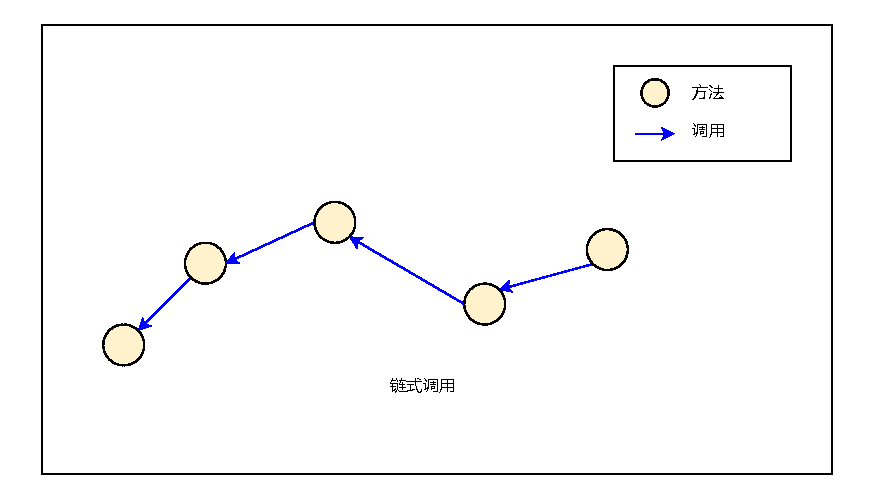
\includegraphics[width = 0.6\textwidth]{figures/链式调用模式图_2.pdf}
\caption{长嵌套调用图模式}
\label{1_长嵌套调用图模式}
\end{figure}




\paragraph{3.复杂方法} 复杂方法的特性之一是职责过多,通常表现为方法内部调用了过多的其他方法、依赖过多的外部变量或与大量方法存在变更影响关系,这种特征在代码审查图中表现为具有大量的出边的中心化节点,如图\ref{1_复杂方法图模式}所示。这种方法的危害有以下几点,1.可维护性差:依赖过多外部方法,任何外部方法的变动都可能导致当前方法的变动,增加维护成本。2.增加耦合度,降低了系统的灵活性。3.违背单一职责原则。

\begin{figure}[h]
\centering
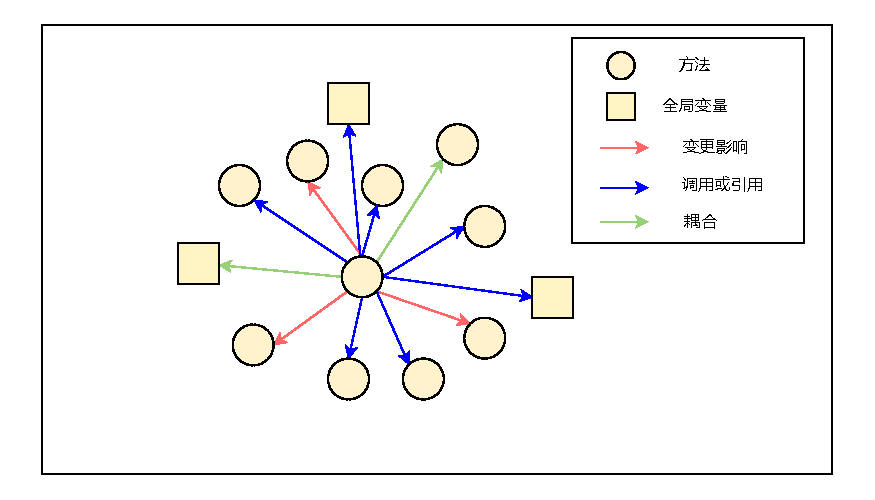
\includegraphics[width = 0.65\textwidth]{figures/3_复杂方法图模式.pdf}
\caption{复杂方法图模式}
\label{1_复杂方法图模式}
\end{figure}



通过代码审查图用户可以迅速定位到复杂方法,深入了解其上下文信息,进而判断其是否存在不合理的复杂度。优化时,用户可以考虑通过方法分解和增加中间层的方式重构该方法、简化其职责并调整其与其他模块的关系,从而有效提升系统的可维护性和可扩展性。


\paragraph{4.职责不匹配} 在软件项目里,每个代码元素都处于特定的物理位置,比如所在的文件、类、文件夹等。这种物理位置往往体现了软件最初的设计理念。而在静态代码结构中,每个代码元素还处于特定的逻辑位置,这在代码审查图中,表现为与其他代码元素的相对位置关系。对于某些方法而言,会出现一种情况:其承担的职责与它所处的物理位置不再完全适配,反而与其他模块的关联更为紧密。我们将这种问题称作职责不匹配问题。

\begin{figure}[h]
\centering
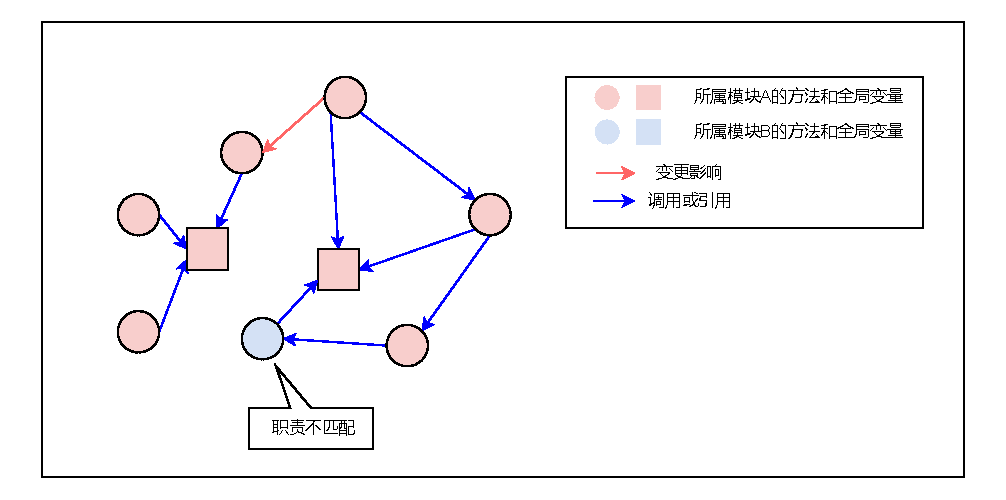
\includegraphics[width = 0.6\textwidth]{figures/职责不匹配_2.pdf}
\caption{职责不匹配图模式}
\label{1_职责不匹配图模式}
\end{figure}

代码审查图中,相同模块的代码元素呈现为同一颜色,不同模块不同颜色,得益于力导向的可视化特性,逻辑上紧密依赖的节点聚集在一起。职责不匹配的特征在代码审查图中的模式如图\ref{1_职责不匹配图模式}所示,表现为逻辑聚集的节点颜色不统一,某些节点(如图\ref{1_职责不匹配图模式}中的蓝色节点)与模块的主色调(红色节点)不符。优化时一般有两种角度,如果用户认可最初的设计理念,可将职责不匹配的代码与主模块进行拆分,如果用户认为逻辑位置更为合适,则可将职责不匹配的代码合并进主模块。通过这样的重构操作,可将依赖和变更影响关系限制在同一模块内,避免变更时跨模块的影响。


\paragraph{5.隐式逻辑型变更模式} 对于软件代码而言,模块间的变更影响关系应当以依赖型变更显式地呈现,这有助于开发者在静态结构中清晰地识别依赖关系。相比之下,逻辑型变更影响往往隐匿在代码内部,仅通过代码上下文或前后调用关系难以察觉。模块间的变更影响通常被视为不利因素,它可能导致不良变更传播问题,需要引起维护人员的关注。

\begin{figure}[h]
\centering
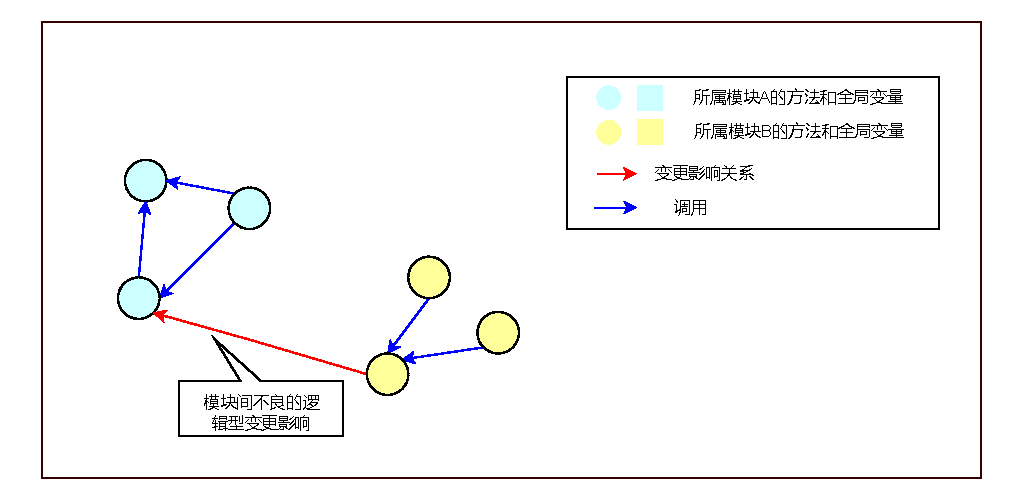
\includegraphics[width = 0.6\textwidth]{figures/4_不良变更影响.pdf}
\caption{隐式逻辑型变更模式}
\label{1_不良的逻辑型变更影响}
\end{figure}


这种隐式逻辑型变更模式在代码审查图中表现为图\ref{1_不良的逻辑型变更影响}所示的模式,其中红色边表示逻辑型变更影响关系,蓝色边表示调用关系。两个模块由于逻辑型影响被连接在一起,导致变更时很难察觉,且模块间互相影响。这种现象暴露了系统架构中的潜在问题——虽然各模块内部结构较为合理,但模块间的依赖关系复杂且紧密,增加了维护和变更时的复杂性与风险。为了解决这一问题,优化的建议是尽量减少或消除这些不良的变更影响关系,或者将其转化为依赖型影响,从而减少隐匿的跨模块变更传播的可能性。

\paragraph{6.模块间紧耦合} 方法间的耦合关系共分为4种,其中公共耦合和外部耦合为耦合性最强的两种,存在显著的缺点。公共耦合指多个方法共享同一全局数据结构,外部耦合是指一组方法通过访问同一全局简单变量进行交互,这两种耦合方式使得方法之间的依赖关系变得隐晦且难以追踪,变量的改变可能引发多个方法的异常行为,且问题的根源往往难以定位。而不同模块间的这两种耦合则更为严重,由于扩散效应,可能导致两个模块间功能逻辑被影响。


\begin{figure}[h]
\centering
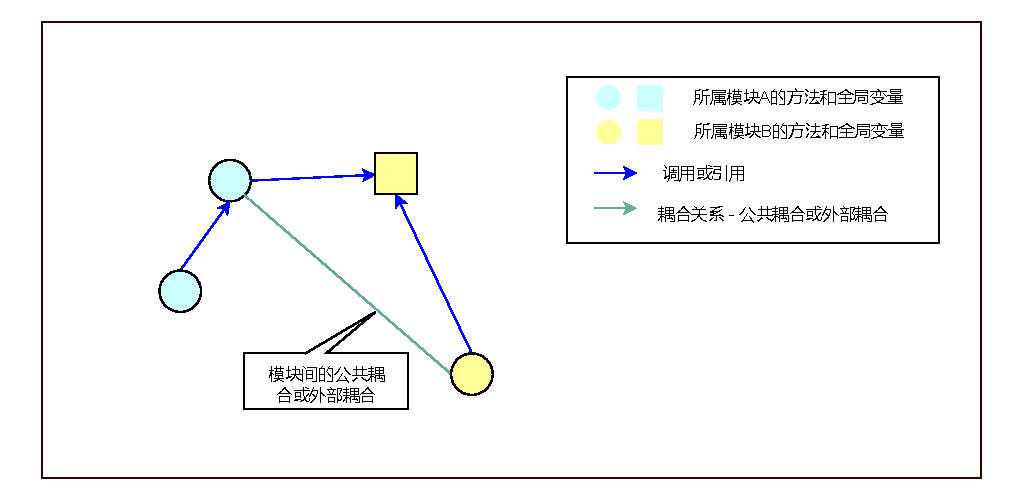
\includegraphics[width = 0.6\textwidth]{figures/4_模块间公共耦合.pdf}
\caption{模块间的公共耦合或外部耦合}
\label{1_模块间的公共耦合或外部耦合}
\end{figure}

这种模块间的公共耦合和外部耦合表现为图\ref{1_模块间的公共耦合或外部耦合}所示的模式,两个所属模块不同的方法被公共耦合或外部耦合类型的边连接起来。在优化时,建议通过参数传递数据,将公共耦合或外部耦合降级为标记耦合或数据耦合,避免直接访问同一全局变量。



\section{代码质量分析报告生成}

在软件开发和代码审查的过程中,开发者可以借助代码审查图聚焦于代码的上下文,帮助发现局部代码的问题。然而,当软件开发完成,开发者希望从全局角度对软件项目的整体质量进行衡量时,仅依靠代码审查图可能会存在质量信息过于分散、不易聚焦的问题。因此,本节进一步通过生成文档化的代码审查报告,为开发者提供统一的代码质量概览,帮助其全面掌握项目的质量状况。

代码审查报告的核心目标是揭示软件项目中存在的关键质量问题,因此本文以提取的代码质量属性与子属性为主线,系统性地向用户报告代码中的相对质量子属性为差的模块或方法,并给出相应的建议。为了帮助用户在代码开发过程中防止变更不完全,报告还将列出项目中所有的代码变更影响关系。用户可以参考这些信息,在变更时全面分析影响范围,降低遗漏风险。

% 通过对这些信息的整合与分析,生成的报告文档为用户提供了一份全面的代码质量概览,既可以帮助用户识别代码中的潜在问题,又能为系统的后续优化与维护提供指导性建议。

\section{实验结果与分析}

\subsection{实验数据和实验设计}

本章实验从软件的历史版本变更角度出发,结合代码度量和不良图模式,探讨在代码历史中修复和重构概率较大的代码与其质量或代码审查图模式之间的关系,从而验证其有效性。

\noindent \textbf{1.实验数据}

本章选取第二章的部分项目进行研究,选择jemalloc为示例项目进行代码质量度量模型的分析实验,选择jemalloc和TheAlgorithms项目进行代码审查图的不良图模式的分析实验。

将项目的历史提交按以下原则进行筛选,筛选后收集提交前版本的项目源代码,提取在该提交中变更的方法,得到<code,list<changed\_func>>的二元组。

\begin{itemize}
    \item 按关键词筛选提交:保留提交信息中包含以下关键词的提交:\{ fix, refactor, Fix, Refactor,improve,Improve \}。这些关键词通常出现在与缺陷修复和代码重构相关的提交中,能在一定程度上反映用户提高代码质量的操作。
    \item 进一步按代码变更类型筛选:分析代码变更,判断是否真正包含修复或重构的行为。
\end{itemize}

\begin{table}[htbp]
\caption{jemalloc-5.3.0数据统计}
\vspace{0.5em}\centering\wuhao
\begin{tabular}{cccccc}
\toprule
项目属性 & 数值/信息 \\
\midrule
总提交 & 3530 \\
包含修复提交 & 653  \\
包含重构提交 & 53  \\
修复提交抽样 & 10 \\
重构提交抽样 &  10 \\
\bottomrule
\end{tabular}
\end{table}

\noindent \textbf{2.验证代码质量度量模型的实验设计}

本实验的核心数据是代码历史版本和对应的提交记录,具体步骤如下:(1)对于实验数据中收集到的提交,对提交前版本的项目源代码进行代码度量计算,不同的质量属性内部进行分档排名,得到方法之间的相对质量关系。(2)将该提交中变更的方法与不同分档进行求交集,得到每档中方法变更的数量。(3)观察代码质量度量和变更概率的数量关系,验证其相关性。如果有一定的相关性,则说明质量度量模型能在一定程度上反映项目中质量较差的代码,帮助用户有针对性地进行优化和重构。

\noindent \textbf{3.验证代码审查图中不良图模式的实验设计}

本实验以实证分析的方式验证不良图模式。(1)针对项目中较为稳定的代码版本,首先生成代码审查图,分析并发现其存在的不良图模式。(2)跟踪后续版本对这些模式的演变情况,尤其是开发者在变更过程中对其进行的重构或修复操作,验证这些不良图模式对软件维护的不利影响,从而进一步证明代码审查图在代码质量评估、优化重构以及开发决策中的指导意义。


\subsection{实验环境}


实验环境如表\ref{4_实验环境}所示。

\begin{table}[htbp]
\caption{实验环境}
\label{4_实验环境}
\vspace{0.5em}\centering\wuhao
\begin{tabular}{cccc}
\toprule
    & 环境 & 版本信息 \\
\midrule
操作系统 & macOS & Ventura v13.5.2  \\
编译环境 & python & 3.7   \\
图可视化环境 & G6 & g6.min.js 4.3.11  \\  
C/C++语言解析环境 & libclang & 15.0.7  \\ 
\bottomrule
\end{tabular}
\end{table}


% 对于代码审查报告的生成,则是验证审查报告的格式是否符合设计方案。

\subsection{实验结果分析}

本节将通过实验和实证分析来验证本章中提出的代码审查图对开发者在代码变更过程中是否有一定的指导作用,这里主要讨论下列两个问题:

RQ1: 代码质量度量与版本历史中修复和重构相关的代码变更是否存在一定的相关性,在修复或重构过程中,代码质量如何影响开发人员的变更行为?

RQ2: 代码审查图中不良图模式与版本历史中修复和重构相关的代码变更是否存在一定的相关性?基于代码审查图的分析能否为代码优化重构提供指导?


\textbf{1.针对于RQ1的实验}

% jemalloc
% 文件206个
% 方法2001个

以\ref{3_代码质量度量模型}节中质量度量模型的质量属性为分析对象,得到的实验结果如图\ref{1_度量模型分析实验}所示,表中横坐标表示代码度量的相对值,横坐标越大,代码质量越好。纵坐标表示在修复或重构的变更历史中,被变更的方法数量比例。

\begin{figure}[h]
\centering
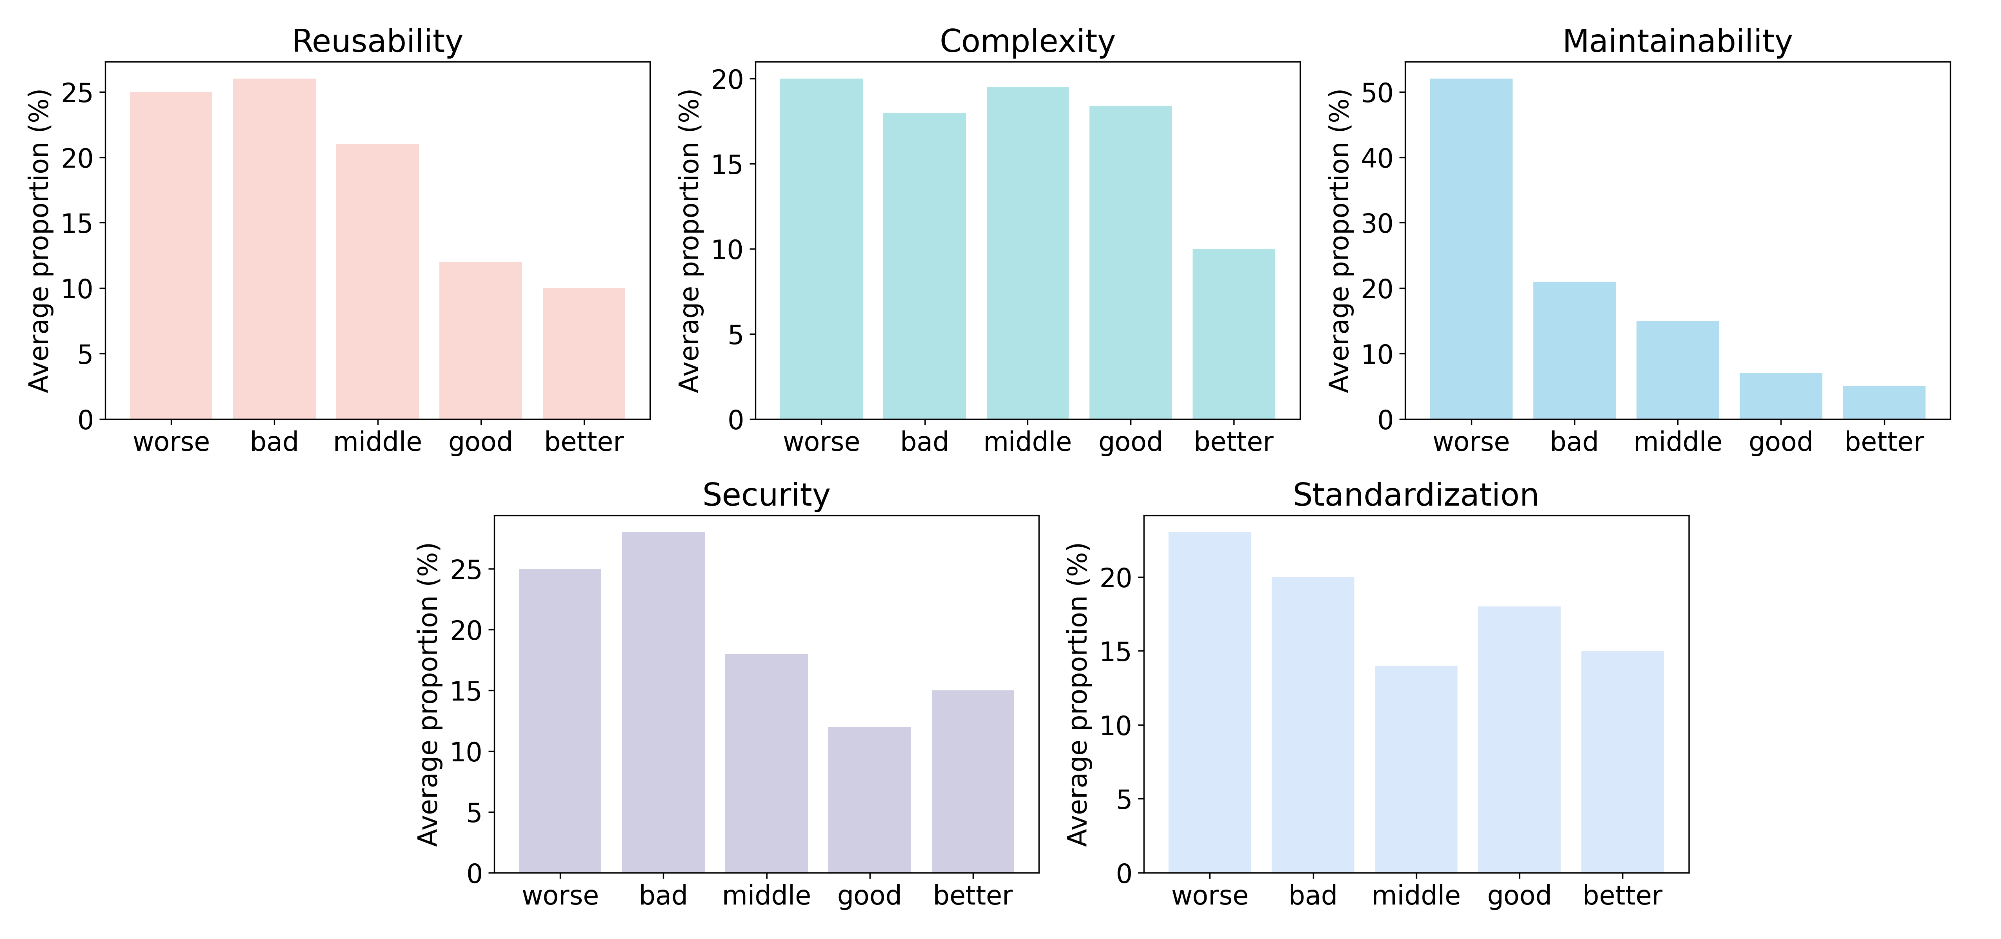
\includegraphics[width = 1\textwidth]{figures/3_度量实验.png}
\caption{代码质量度量 - 方法变更比例}
\label{1_度量模型分析实验}
\end{figure}


通过图\ref{1_度量模型分析实验}可以看出,在修复或重构等操作过程中,大多数变更都集中在代码度量较差的部分。这表明,度量较差的代码相较于度量较好的代码,在重构或修复的提交中更容易被修改。

进一步分析可以发现,这种现象在可维护性上表现最为明显。可维护性较差的代码具有更大范围的变更影响和更强的耦合性,对质量子属性进一步分析,发现可维护性较差的代码中大部分集中在耦合性更强的方法上,如图\ref{4_子属性}所示。说明在实际开发过程中,开发者更倾向于优化这类代码,以减少未来维护过程中因代码结构混乱而带来的修改成本,还能提高代码的可读性、清晰度和模块化程度,从而有效降低长期维护的风险和成本。

其次是可复用性和安全性。可复用性较差的代码具有较高的耦合度、低内聚性或高扇出低扇入,使其难以在不同模块或项目中直接复用。重构的变更在扇出对应的质量子属性上表现更加明显,如图\ref{4_子属性}所示。为了提高代码的复用价值,开发者往往会在重构过程中拆分模块、减少冗余或提升通用性,使其能够适应更多场景,从而降低开发成本。而安全性较差的代码存在往往存在安全漏洞,可能导致系统遭受攻击等严重后果,因此也被开发者所重视。

\begin{figure}[h]
\centering
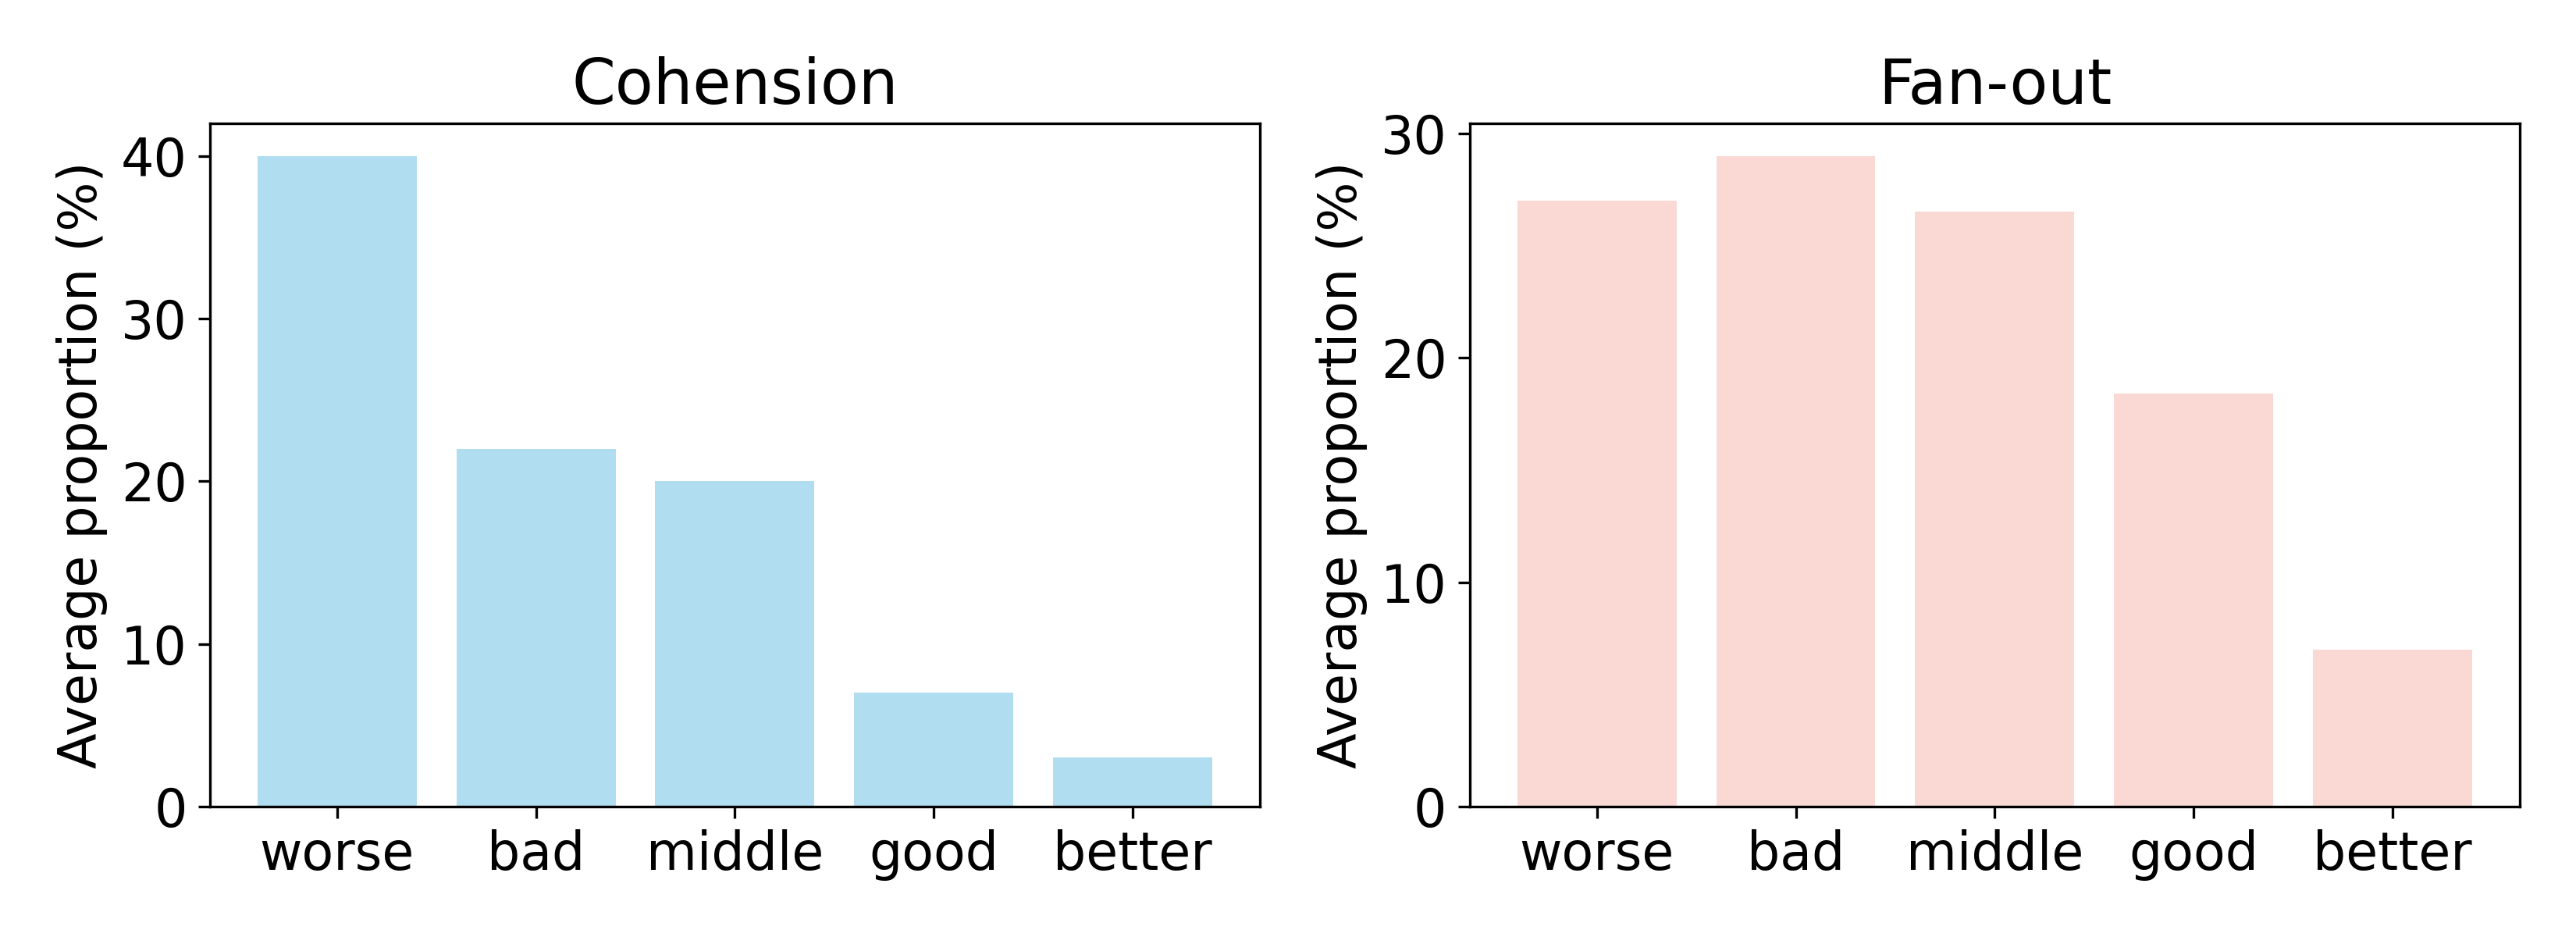
\includegraphics[width = 0.7\textwidth]{figures/4_子属性.jpg}
\caption{质量子属性度量(耦合性和扇出) - 方法变更比例}
\label{4_子属性}
\end{figure}

而在复杂性和规范性上则没有明显的趋势。对于复杂性而言,原因可能是不同的开发人员对于代码复杂性的感知和接受程度可能有所不同,并且在某些情况下,复杂性高的代码并不一定意味着它就需要被优先重构或修复,因为其可能是为了实现特定的性能要求或者业务逻辑而有意为之。对于规范性而言,它更多地侧重于代码是否遵循了特定的编码标准和风格指南,虽然不规范的代码可能会给团队协作和后续的维护带来一定的麻烦,但在某些情况下,不影响代码功能和性能的轻微不规范问题可能会被暂时搁置,开发人员更倾向于优先处理那些会直接影响系统可维护性、可复用性和安全性的代码部分。

这些现象也从侧面反映出开发人员在进行代码重构和修复工作时,往往会优先考虑那些对系统的长期稳定性和扩展性有重要影响的代码属性,可维护性、可复用性和安全性方面的问题一旦出现,会对系统的可靠性和后续开发造成更大的潜在风险,因此更容易受到关注和处理;而对于复杂性和规范性,由于其在某些情况下的模糊性和非紧急性,在代码的重构和修复过程中没有像其他属性那样呈现出明显的变更趋势。

因此,开发者在软件开发或维护过程中,应当更加关注代码的可维护性、安全性以及可复用性。更深入来讲,需留意模块的内聚性、方法的扇入扇出,避免产生过紧的耦合,并尽量减少逻辑型的变更影响,同时也要确保代码的安全性。在处理质量分析报告时,应将涉及这三类的问题赋予较高的优先级。

上述实验结果反过来也验证了代码质量度量模型在实际应用时的指导意义,它能够在项目中识别出质量较差的代码区域,从而帮助开发人员优先关注这些部分,在提升整体代码质量时有针对性地进行优化和重构。因此,代码质量模型不仅提供了对现有代码质量的量化评估,还能为项目团队提供具体的优化方向,确保资源投入最大化地改善代码质量。

\textbf{2.针对于RQ2的实证分析}

本实验的基本思想是通过分析项目代码某一版本的代码审查图,发现其不良图模式,观察后续版本中对该不良图模式的变更,尤其是重构或修复的行为,从而验证其不良性,进而验证代码审查图对代码质量分析和优化重构的指导意义。针对4.4节总结的不良图模式,在示例项目(TheAlgorithms项目和jemalloc项目)中均出现过对应子图,并且在后续版本的优化中,存在不同程度的重构、变更或优化。

\begin{figure}[!h]
    \setlength{\subfigcapskip}{-1bp}
    \centering
    \begin{minipage}{\textwidth}
    \centering
    \subfigure[冗余代码-jemalloc项目]{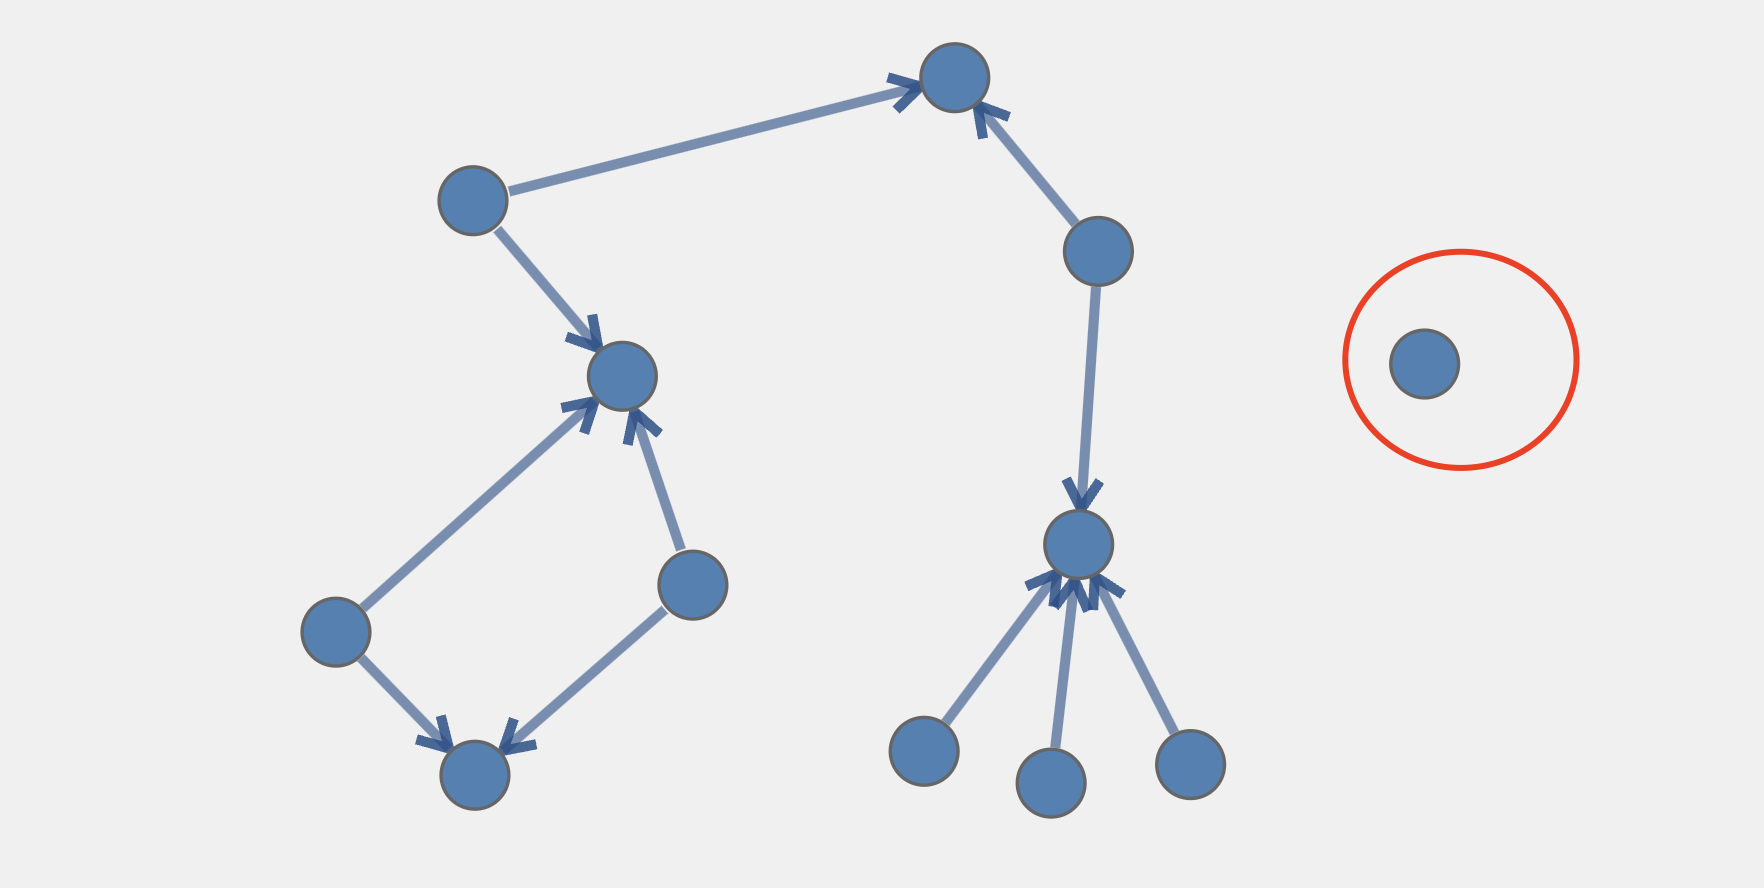
\includegraphics[width=0.4\textwidth]{figures/孤立节点.jpg}} % 保留中文标题
    \hspace{2em}
    \subfigure[长嵌套调用-TheAlgorithms项目]{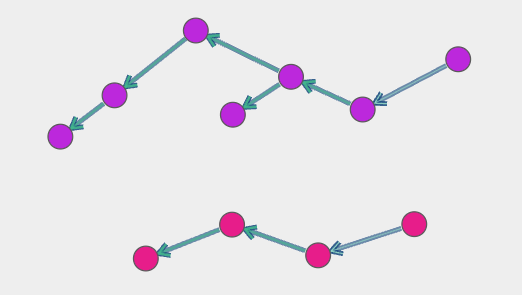
\includegraphics[width=0.4\textwidth]{存在链式调用.jpg}} % 保留中文标题
    \end{minipage}
    \centering
    \begin{minipage}{\textwidth}
    \centering
    \subfigure[复杂方法-jemalloc项目]{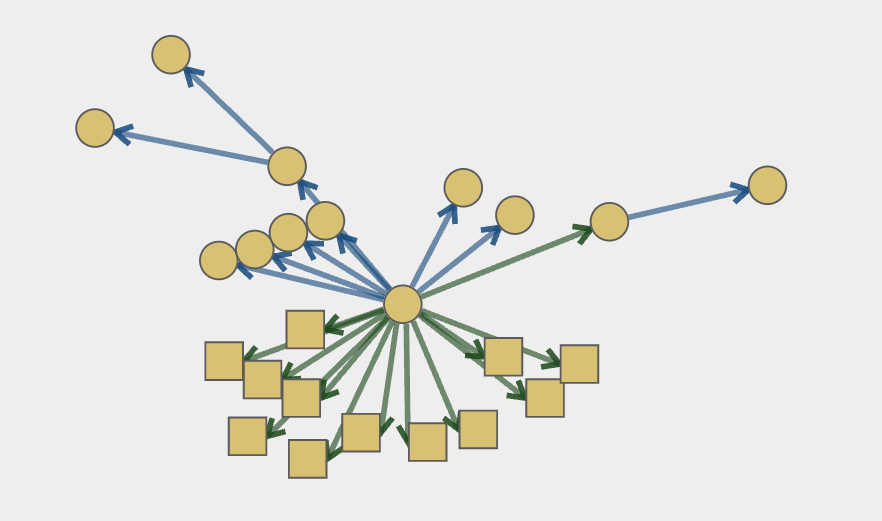
\includegraphics[width=0.4\textwidth]{figures/复杂方法实例.jpg}} % 保留中文标题
    \hspace{2em}
    \subfigure[职责不匹配-jemalloc项目]{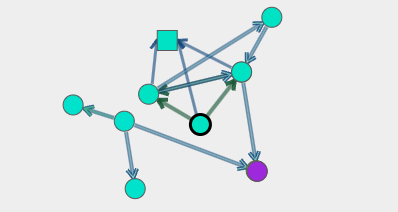
\includegraphics[width=0.4\textwidth]{figures/职责不匹配实例.jpg}} % 保留中文标题
    \end{minipage}
    \vspace{0.2em}
    \caption{示例项目中不良图模式实例} % 只保留中文标题
\end{figure}



图(a)是jemalloc项目5.3.0版本中的实际存在的子图,该图为src/pa.c文件的代码审查图子图。该文件定义了多个方法,从图中可以清晰地看出该文件中方法pa\_shard\_retain\_grow\_limit\_get\_set并未与任何方法产生联系,因此属于冗余代码。在后续的优化中(commit da66aa3),该方法被删除。同时可以观察到该文件的结构较为松散,缺乏足够的联系和协调关系,这种结构也导致了其内聚度较差。仅依靠代码或文字难以直接反映问题,而配合代码审查图,可以更加直观地展示该模块的结构问题。

图(b)是TheAlgorithms项目中numerical\_methods/ode\_midpoint\_euler.c文件和numerical\_methods/ode\_forward\_euler.c文件的部分子图,这两个文件内均出现了长嵌套调用,当中间任何一个方法产生变更时,都可能导致上下游的方法跟着改变,因此变更较为频繁。在提交8513174中对其进行了结构上的优化,使其具有更优的模块化结构。

图(c)是jemalloc项目中5.1.0版本unit/emitter.c文件存在的复杂方法emit\_modal,该方法调用了8个其他方法和12个全局变量,导致其在外部方法变更的同时也要随之变更,因此较为频繁地出现变更行为。在后续的优化中,该方法调用的其他方法进行了组合和重构,该提交eb261e5被收录在v5.2.0中。

图(d)是jemalloc项目中src/hpa.c文件声明的方法hpa\_supported,在5.3.0版本前它并未与其所在文件的其他方法产生联系,而是更多地服务于unit/hpa\_background\_thread.c等文件的方法,因此出现了职责不匹配的现象。该现象在v5.3.0版本有所改善,部分文件外方法与该方法进行了解耦,在如d93eef2等提交中对其增加了文件内方法的调用,使其更专注于本文件内部逻辑。

\begin{figure}[!h]
    \setlength{\subfigcapskip}{-1bp}
    \centering
    \begin{minipage}{\textwidth}
    \centering
    \subfigure[模块间不良的逻辑型变更影响-TheAlgorithms项目]{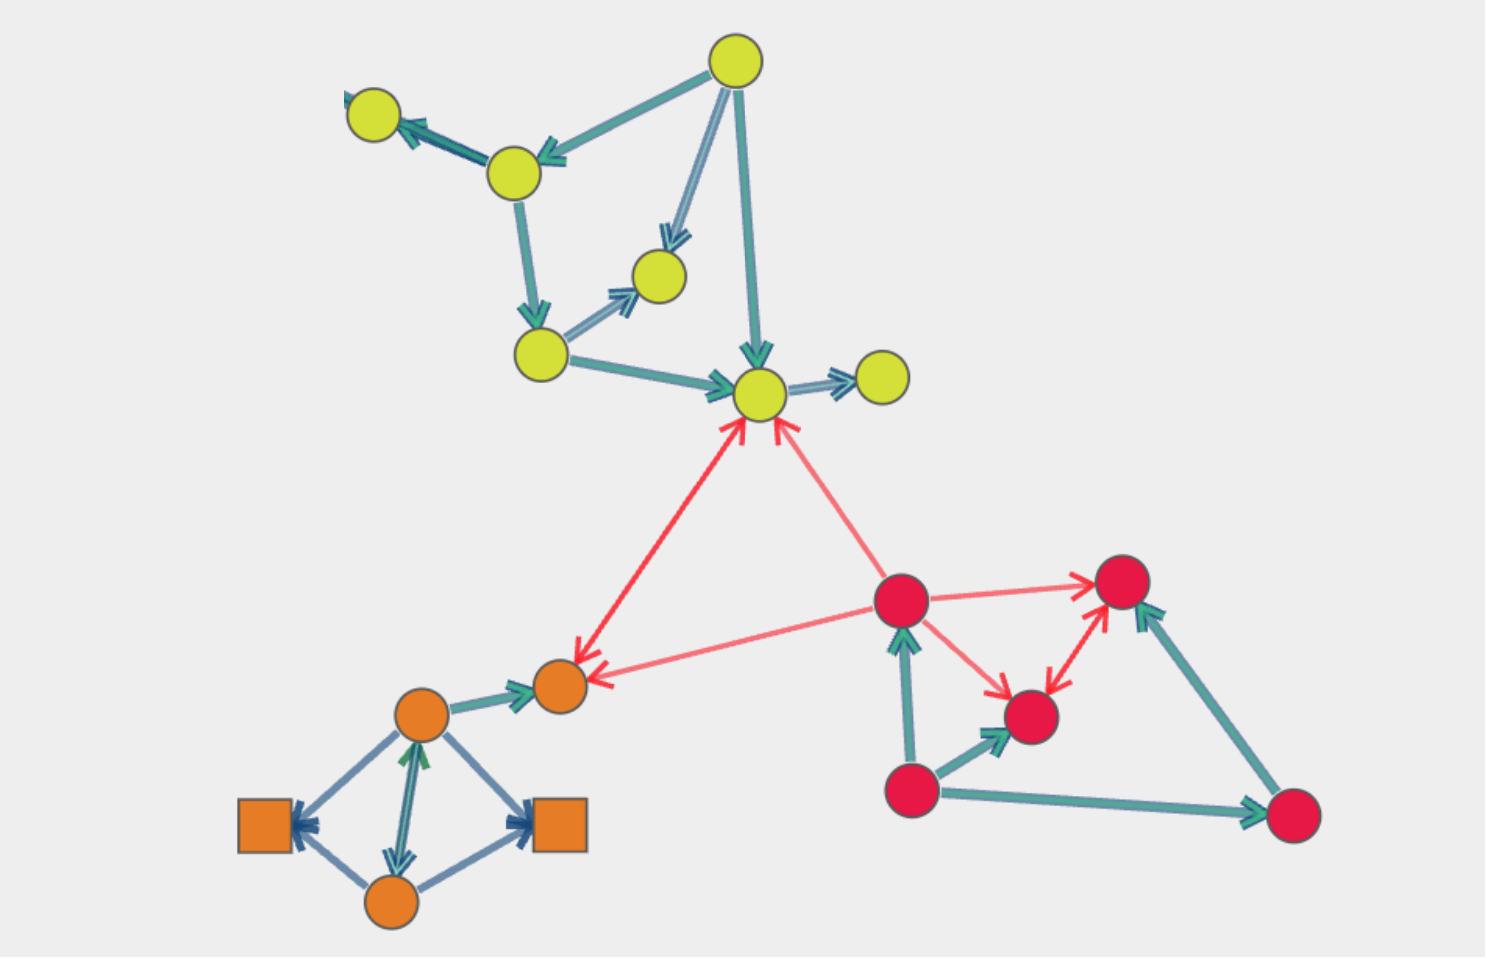
\includegraphics[width=0.4\textwidth]{figures/不良变更影响.png}} % 保留中文标题
    \hspace{2em}
    \subfigure[模块间的不良耦合-jemalloc项目]{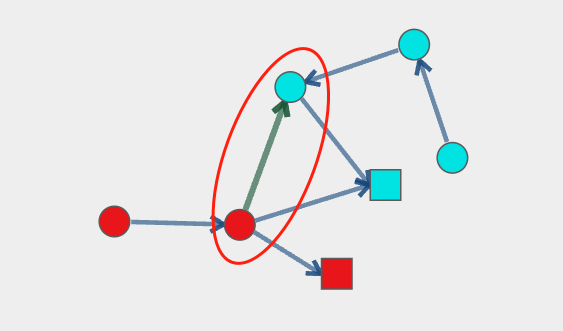
\includegraphics[width=0.4\textwidth]{figures/不良耦合.jpg}} % 保留中文标题
    \end{minipage}
    \vspace{0.2em}
    \caption{代码审查图} % 只保留中文标题
    \label{1_不良的逻辑型变更影响实例}
\end{figure}

图\ref{1_不良的逻辑型变更影响实例}(a)展示了TheAlgorithms项目中的一个实际子图,涉及三个模块,分别是modified\_Binary\_Search、radix\_sort\_2和lexicographic\_Permutations.c。尽管每个模块的内部结构良好,但各有方法与其他模块存在逻辑型影响。因此当这些方法发生变动时,不仅当前模块代码需要修改,其他模块代码也被影响。更严重的是,随着涟漪效应,这些变更可能扩展并影响更多的代码,导致不必要的连锁反应。在后续的4b07f0f等提交中均观察到其同时变更的维护工作。

图\ref{1_不良的逻辑型变更影响实例}(b)中展示了jemalloc项目中的src/decay.c文件与hpa.c文件的部分代码审查图,两个模块由于全局变量h\_steps而产生了外部耦合,这是一种不良的模块间的耦合关系,一个模块内任何改变该变量的操作都可能沿着耦合影响到另一个模块。在v5.2.0中将此种耦合进行了优化,在8229cc7提交中缩小了该变量的作用域,从全局可使用变为了仅在文件内可使用。


因此,通过代码审查图,不仅能够帮助开发者快速定位模块质量问题,还能直观地理解问题的根源,为后续的优化和改进提供清晰的建议。这种结合文字与图形的分析方式,显著提升了代码质量分析的直观性和说服力。


\section{代码审查图的应用案例分析}

代码审查图在实际使用时可以有以下三种用法,分别是作为一种静态分析工具对软件代码进行结构可视化和质量分析、作为一种开发工具辅助开发者的代码维护以及作为一种审查工具帮助审查者进行代码审查。

\noindent \textbf{1.作为一种静态分析工具对软件代码进行结构可视化和质量分析} 

用户可将代码生成代码审查图,观察代码结构。图\ref{4_代码审查图}展示了 Antiword-0.37 项目和 TheAlgorithms 项目的代码审查图。

\begin{figure}[!h]
    \setlength{\subfigcapskip}{-1bp}
    \centering
    \begin{minipage}{\textwidth}
    \centering
    \subfigure[antiword-未划分模块]{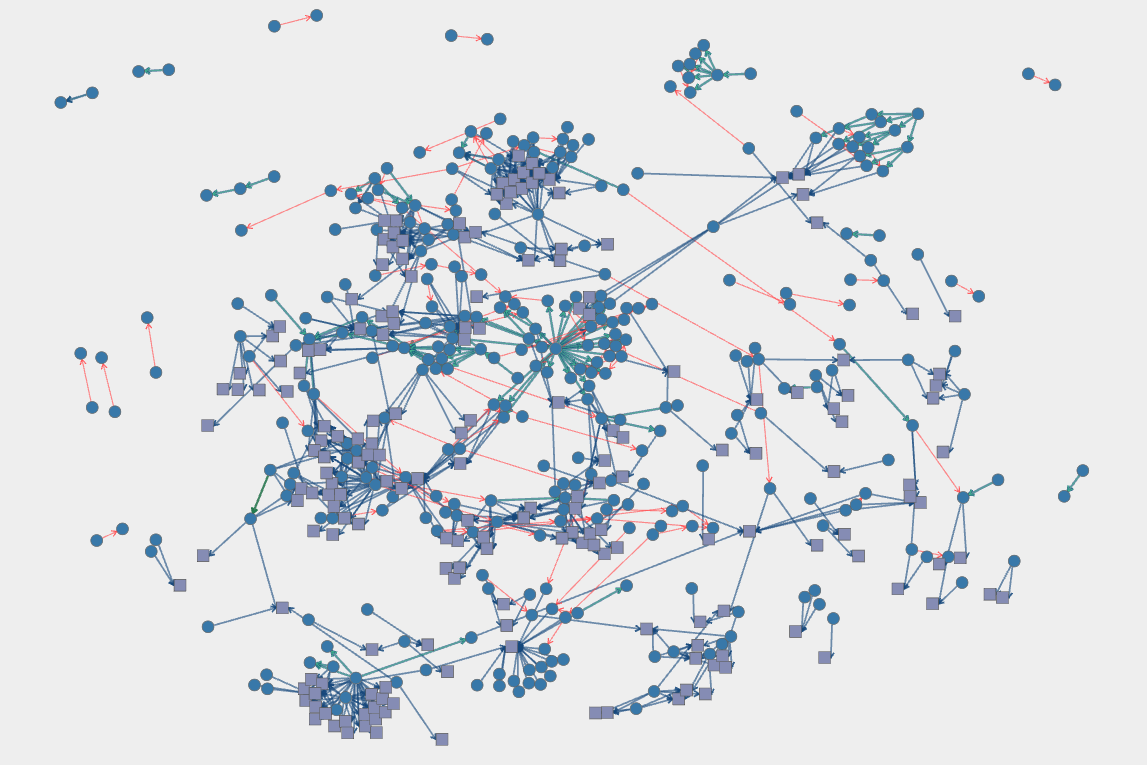
\includegraphics[width=0.4\textwidth]{antiword审查图未上色.jpg}} % 保留中文标题
    \hspace{2em}
    \subfigure[TheAlgorithms-未划分模块]{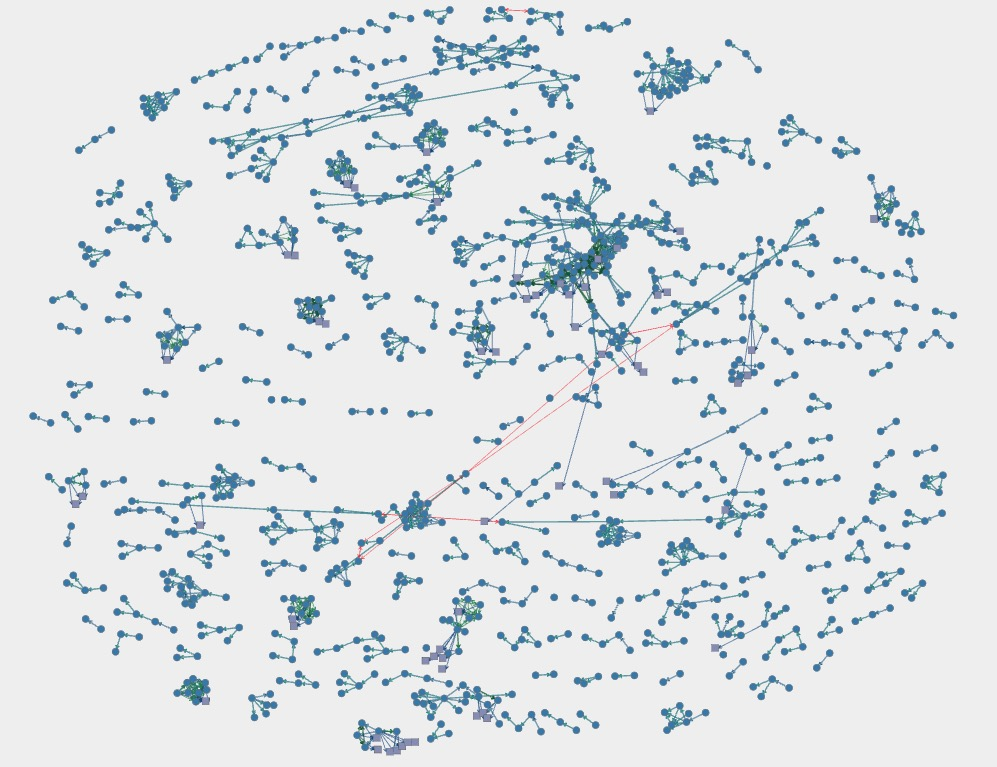
\includegraphics[width=0.4\textwidth]{aigri代码审查图-未上色.jpg}} % 保留中文标题
    \end{minipage}
    \centering
    \begin{minipage}{\textwidth}
    \centering
    \subfigure[antiword-划分模块]{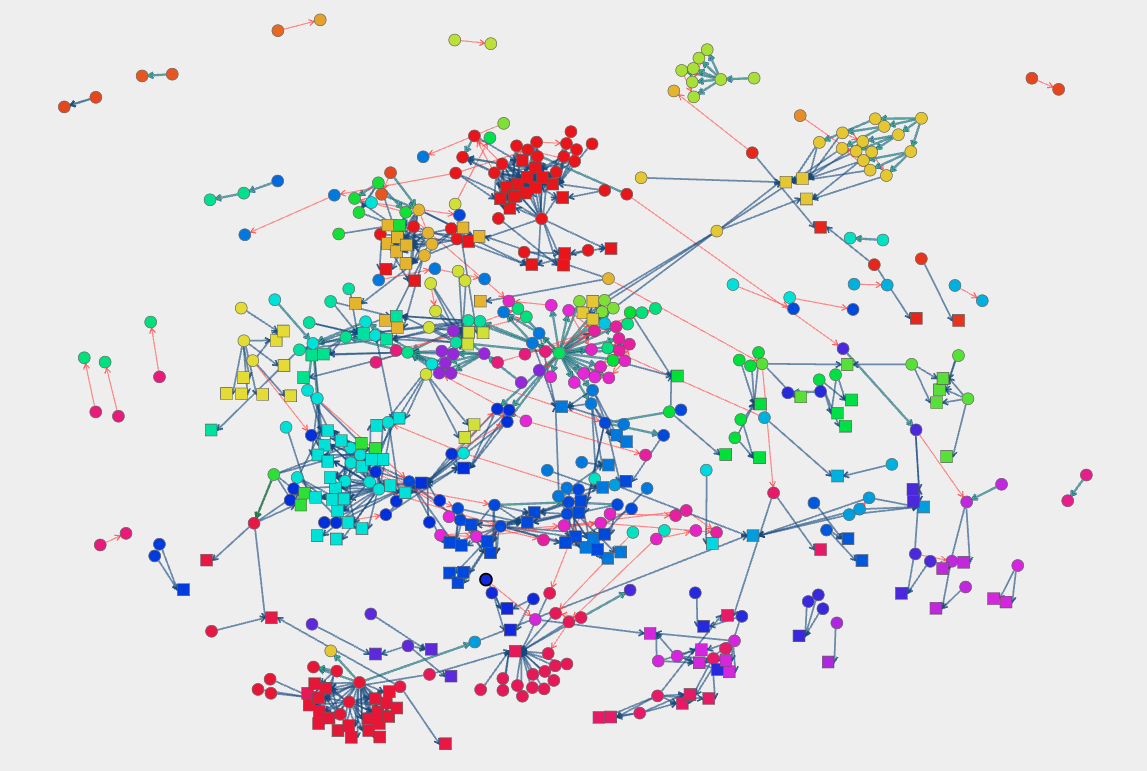
\includegraphics[width=0.4\textwidth]{antiword代码审查图.jpg}} % 保留中文标题
    \hspace{2em}
    \subfigure[TheAlgorithms-划分模块]{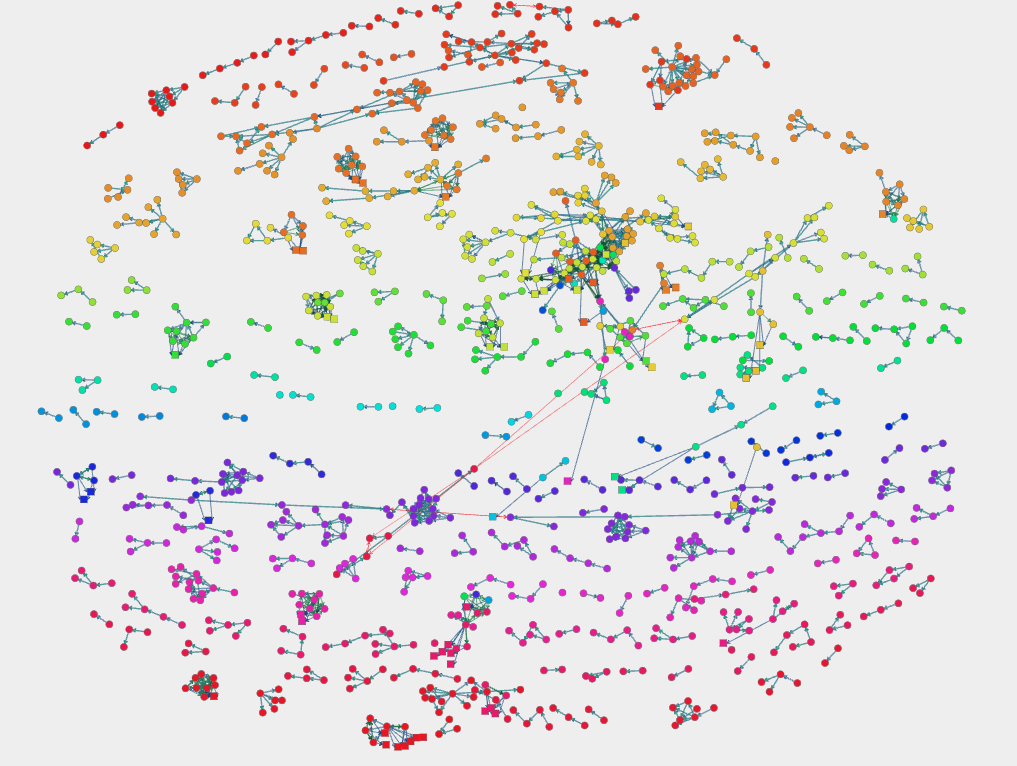
\includegraphics[width=0.4\textwidth]{aigri代码审查图.jpg}} % 保留中文标题
    \end{minipage}
    \vspace{0.2em}
    \caption{代码审查图} % 只保留中文标题
    \label{4_代码审查图}
\end{figure}


图中圆形节点表示方法,方形节点表示全局变量,不同颜色的边则代表了代码元素之间的不同关系:蓝色边表示依赖关系,绿色边表示耦合关系,红色边表示代码变更影响关系。图a和图b是未区分模块的全局视图,体现了代码结构上的相互关联关系。图c和图d则对模块进行了区分,采用颜色区分不同模块,将属于同一模块的节点用相同颜色进行标注,从而进一步突出模块之间的边界和逻辑关系。

\noindent(1)分析结构特征信息

从图中可以明显看出两个项目在代码结构特征上的显著差异。
\begin{itemize}
    \item Antiword 项目整体模块之间高度协作,共同实现一个完整的功能,因此模块之间的联系较为紧密。从可视化图上观察,按模块划分后,可以清晰地看到具有相同功能的模块形成了较为紧密的聚集。同一颜色的节点集中分布,进一步体现了模块的内聚性较高以及逻辑结构的清晰性。
    
    \item TheAlgorithms 项目由于其作为算法库的特性,方法之间的耦合性较低,各模块间的联系相对较弱。从图上来看,不同模块呈现出较为分散的分布,模块内部的聚集程度也较低。整体结构表现为由若干独立模块组成,松散而分离,符合库函数式项目的典型特征。
\end{itemize}

\noindent(2)查看代码度量

\begin{figure}[h]
\centering
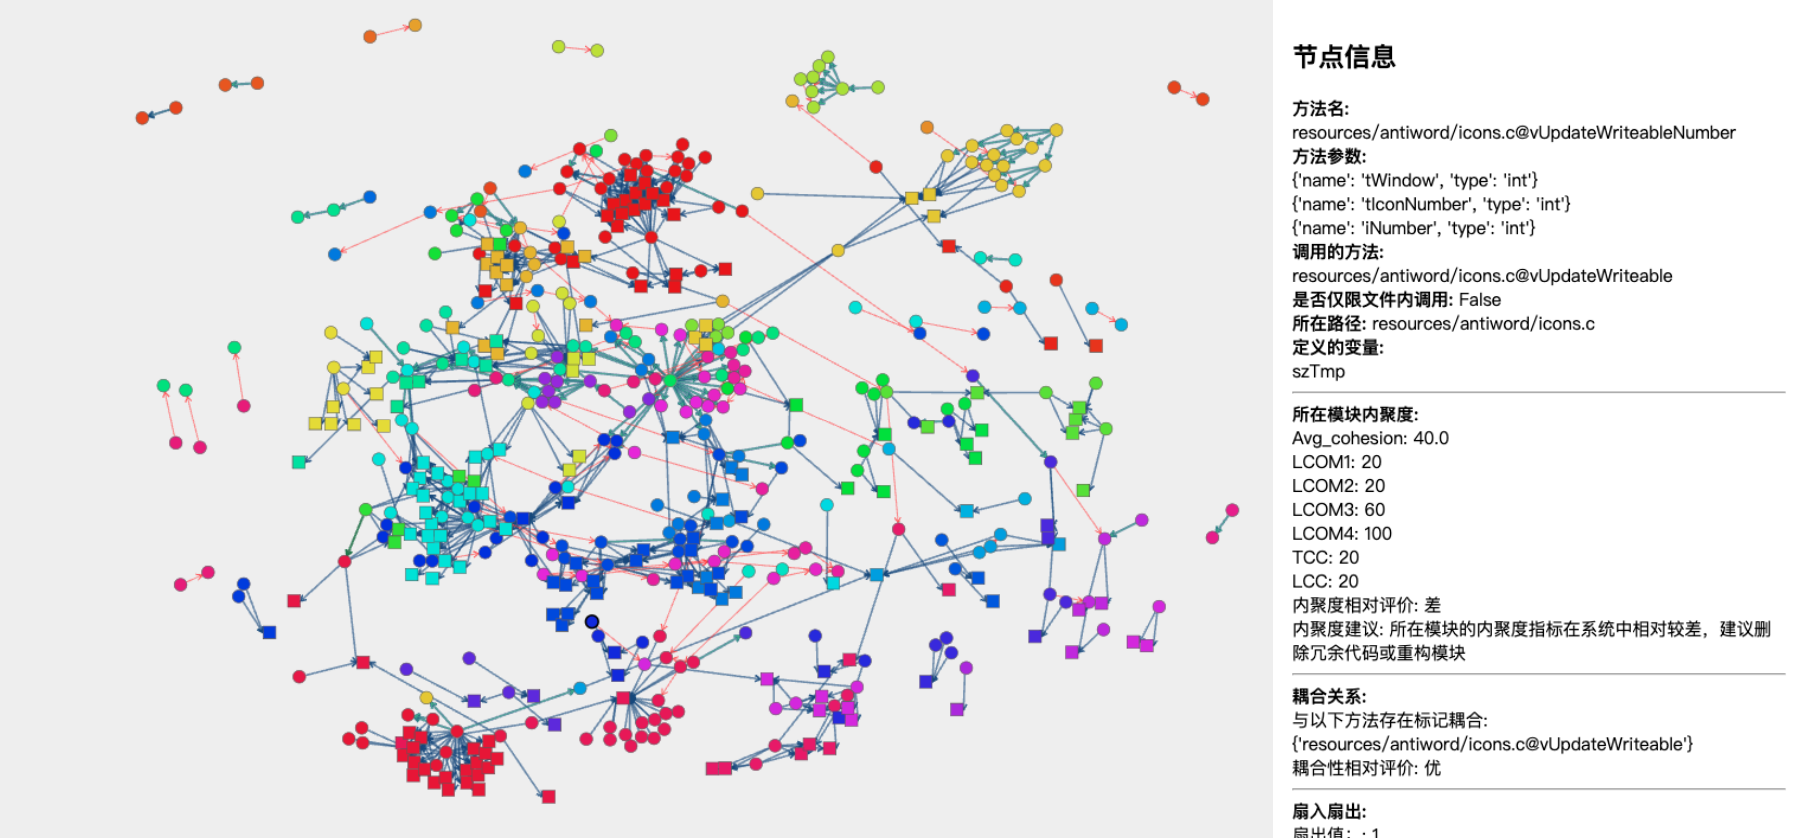
\includegraphics[width = 1\textwidth]{figures/点击节点查看.png}
\caption{点击节点展开节点信息}
\label{4_查看度量}
\end{figure}

 点击图中的某个节点可查看该节点的详细信息,包括方法或全局变量的具体描述,以及代码度量信息,如图\ref{4_查看度量}所示。这一功能能够帮助用户快速了解特定方法或变量的功能和用途,并根据代码度量信息了解方法或所在模块的质量情况,从而更高效地进行代码审查和理解。

\noindent(3)分析不良的图模式

根据\ref{4_不良图模式}中所述的不良图模式,分析Antiword项目的代码审查图,可发现一些对应的子图,如图\ref{4_不良示例}所示,反映了代码中存在的一些质量或结构问题。


\begin{figure}[!h]
    \setlength{\subfigcapskip}{-1bp}
    \centering
    \begin{minipage}{\textwidth}
    \centering
    \subfigure[冗余代码 - misc.c文件内的冗余方法]{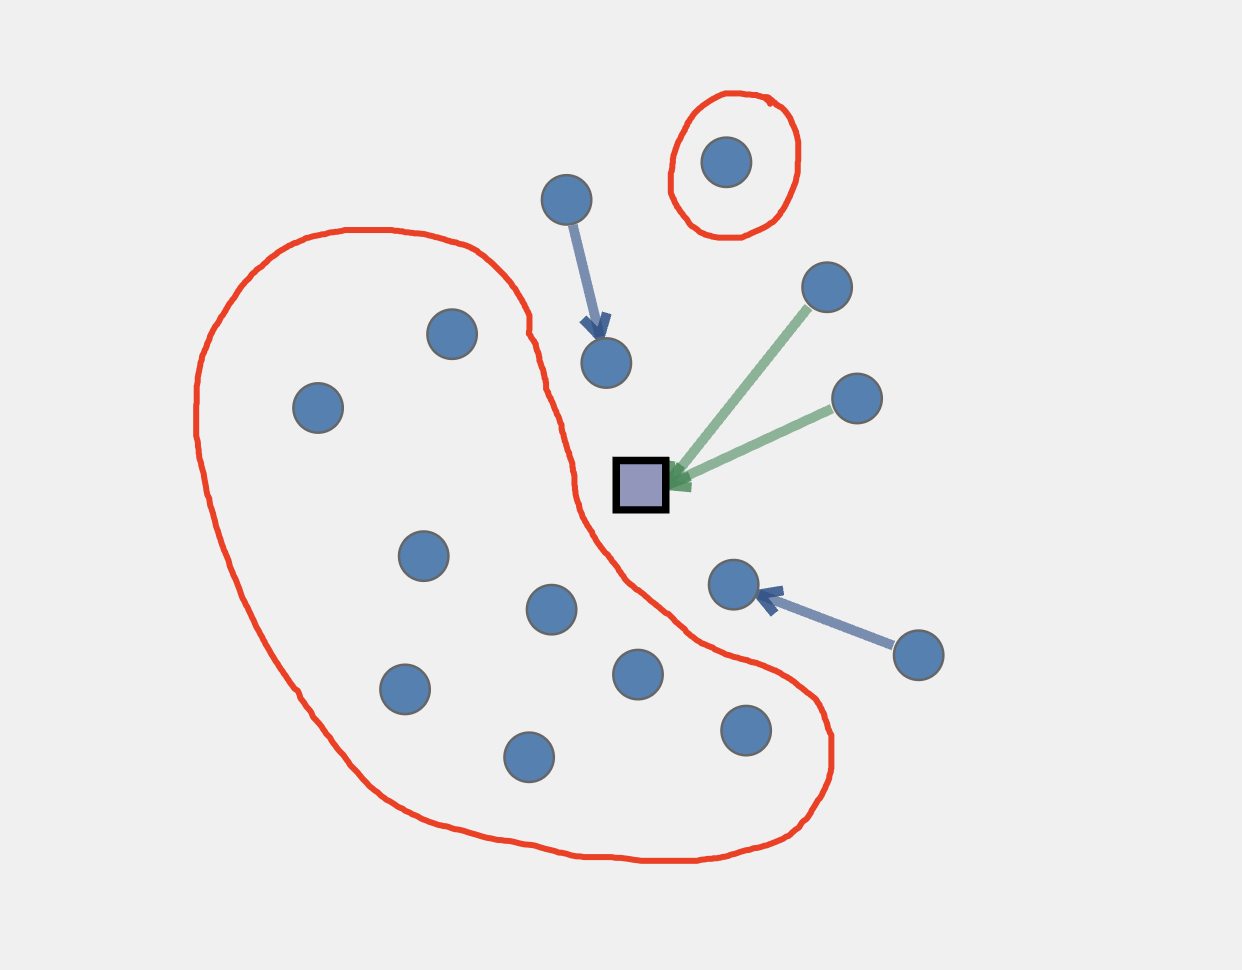
\includegraphics[width=0.4\textwidth]{figures/孤立节点实例.jpg}} % 保留中文标题
    \hspace{2em}
    \subfigure[复杂方法 - properties.c文件中vGetPropertyInfo方法,扇出度30]{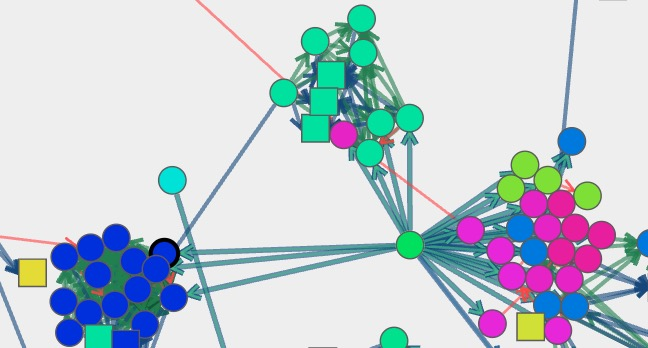
\includegraphics[width=0.4\textwidth]{figures/扇出度最高.jpg}} % 保留中文标题
    \end{minipage}
    \centering
    \begin{minipage}{\textwidth}
    \centering
    \subfigure[职责不匹配 - notes.c中vPrepareFootnoteText方法]{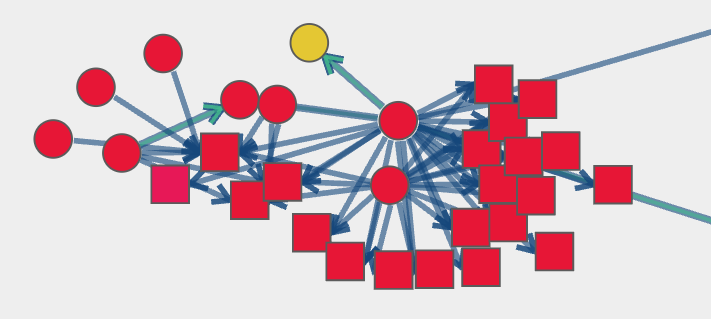
\includegraphics[width=0.4\textwidth]{figures/职责不匹配.png}} % 保留中文标题
    \hspace{2em}
    \subfigure[模块间不良的逻辑型影响-stylelist.c中方法pGetNextStyleInfoListItem和fontlist.c中方法pGetNextFontInfoListItem的克隆型影响]{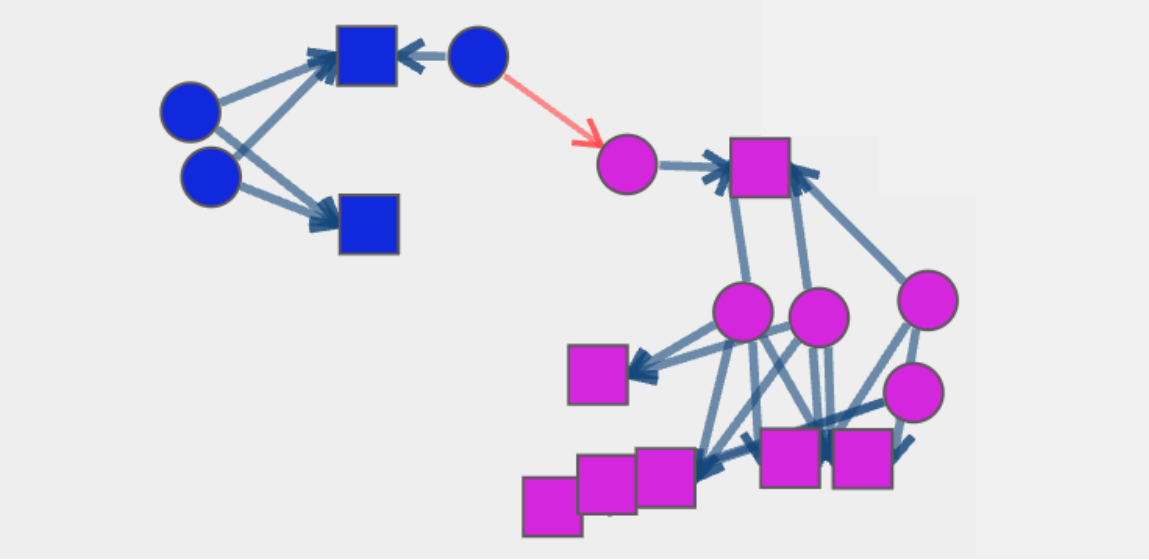
\includegraphics[width=0.4\textwidth]{figures/不良变更影响关系.png}} % 保留中文标题
    \end{minipage}
    \vspace{0.2em}
    \caption{antiword代码审查图中的部分不良子图} % 只保留中文标题
    \label{4_不良示例}
\end{figure}

\noindent(4)导出质量分析报告

图\ref{4_报告节选}展示了一个实际的代码分析报告示例。由于报告内容较长,这里仅展示了其中的一部分信息。通过代码分析报告,用户能够以结构化的清单形式全面了解软件项目中存在的各类质量问题及其具体位置。这些报告不仅清晰地列出了每个问题的详细描述,还提供了针对性优化或重构的建议。通过这种方式,开发团队可以快速识别代码中的潜在缺陷或性能瓶颈,并根据报告中提供的指导意见,采取有效的措施进行改进。报告的可视化和条目化呈现,帮助用户直观地理解各项问题的优先级和重要性,从而优化项目的维护流程,并提高软件系统的整体质量。

\begin{figure}[h]
\centering
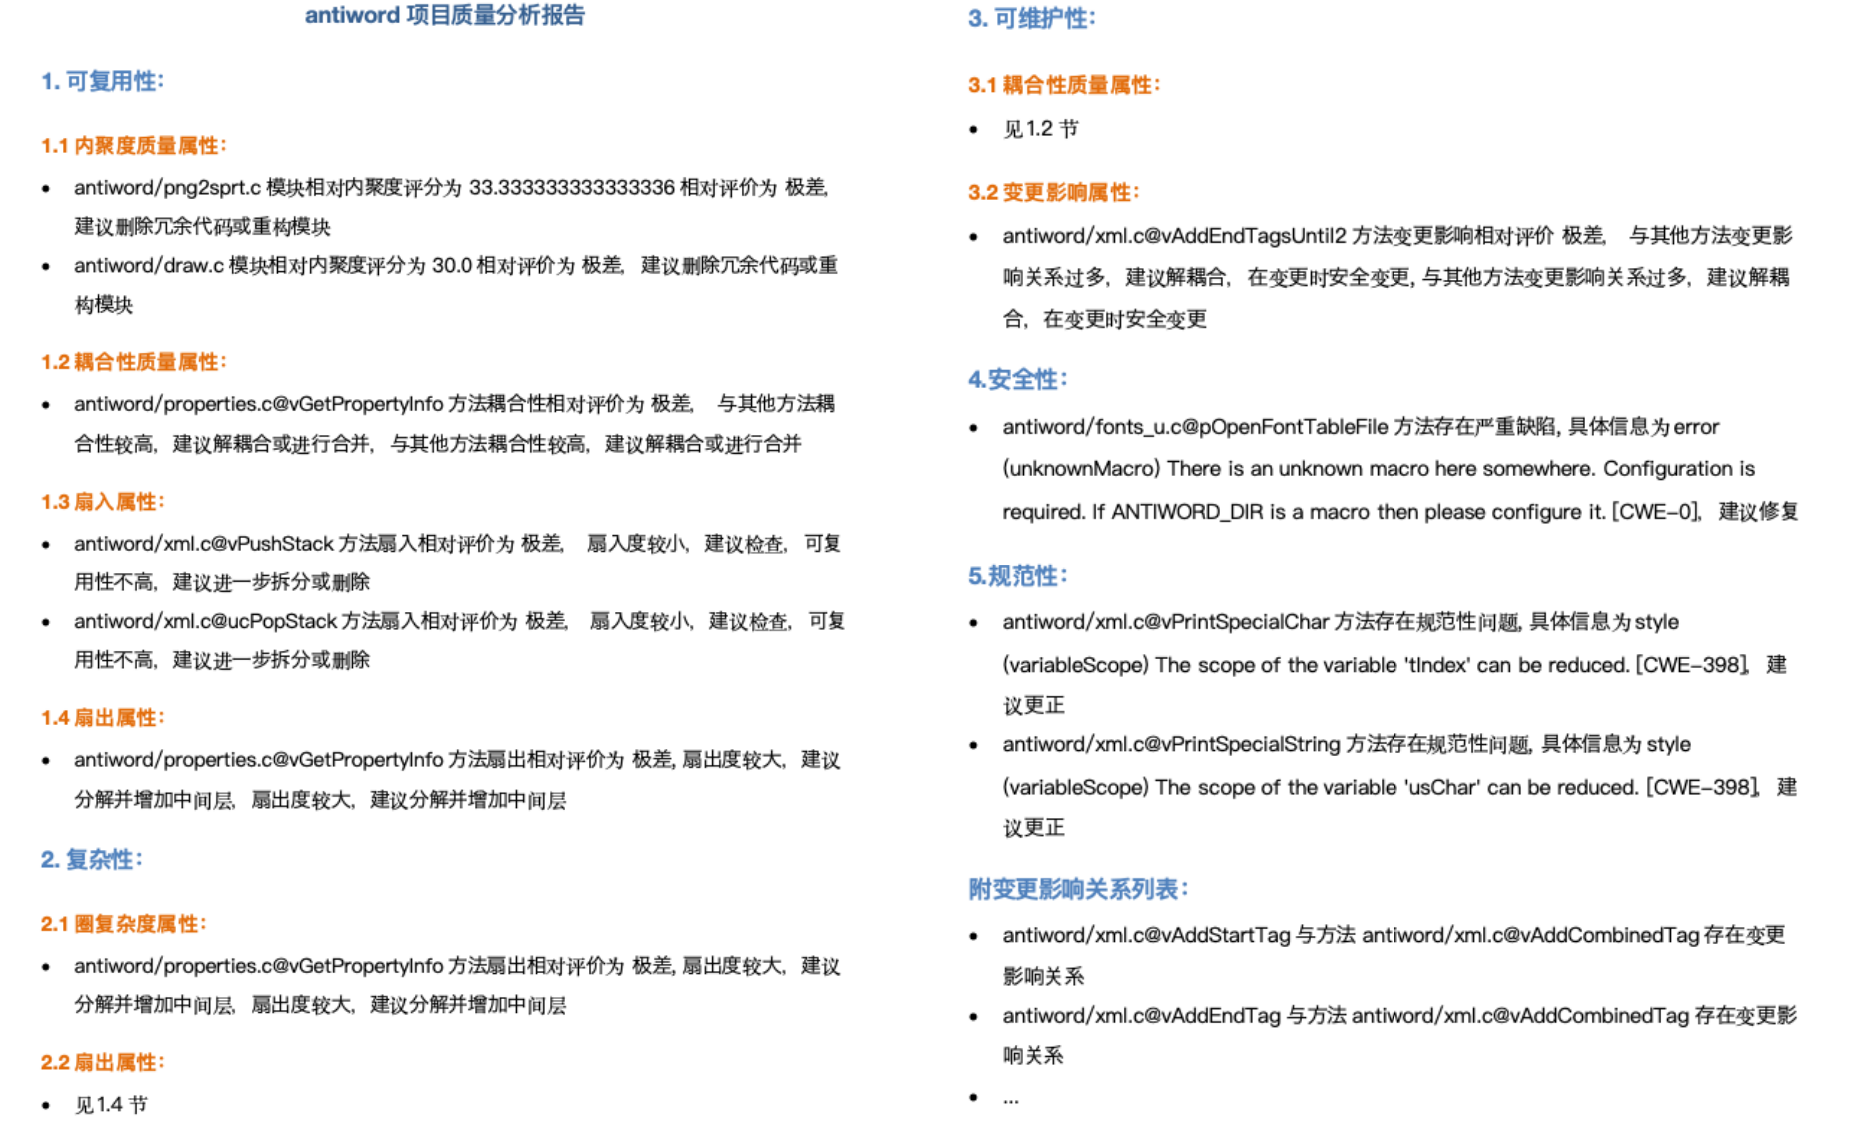
\includegraphics[width = 1.0\textwidth]{figures/报告.png}
\caption{antiword项目代码质量分析报告节选}
\label{4_报告节选}
\end{figure}


\noindent \textbf{2.作为一种开发工具辅助开发者的代码维护} 

当用户对软件代码进行开发时,也可按以下步骤辅助代码维护。

\noindent(1)将复杂庞大的项目先通过系统进行分析,得到对应的代码审查图,如图\ref{1_导入项目生成代码审查图}所示。

\begin{figure}[h]
\centering
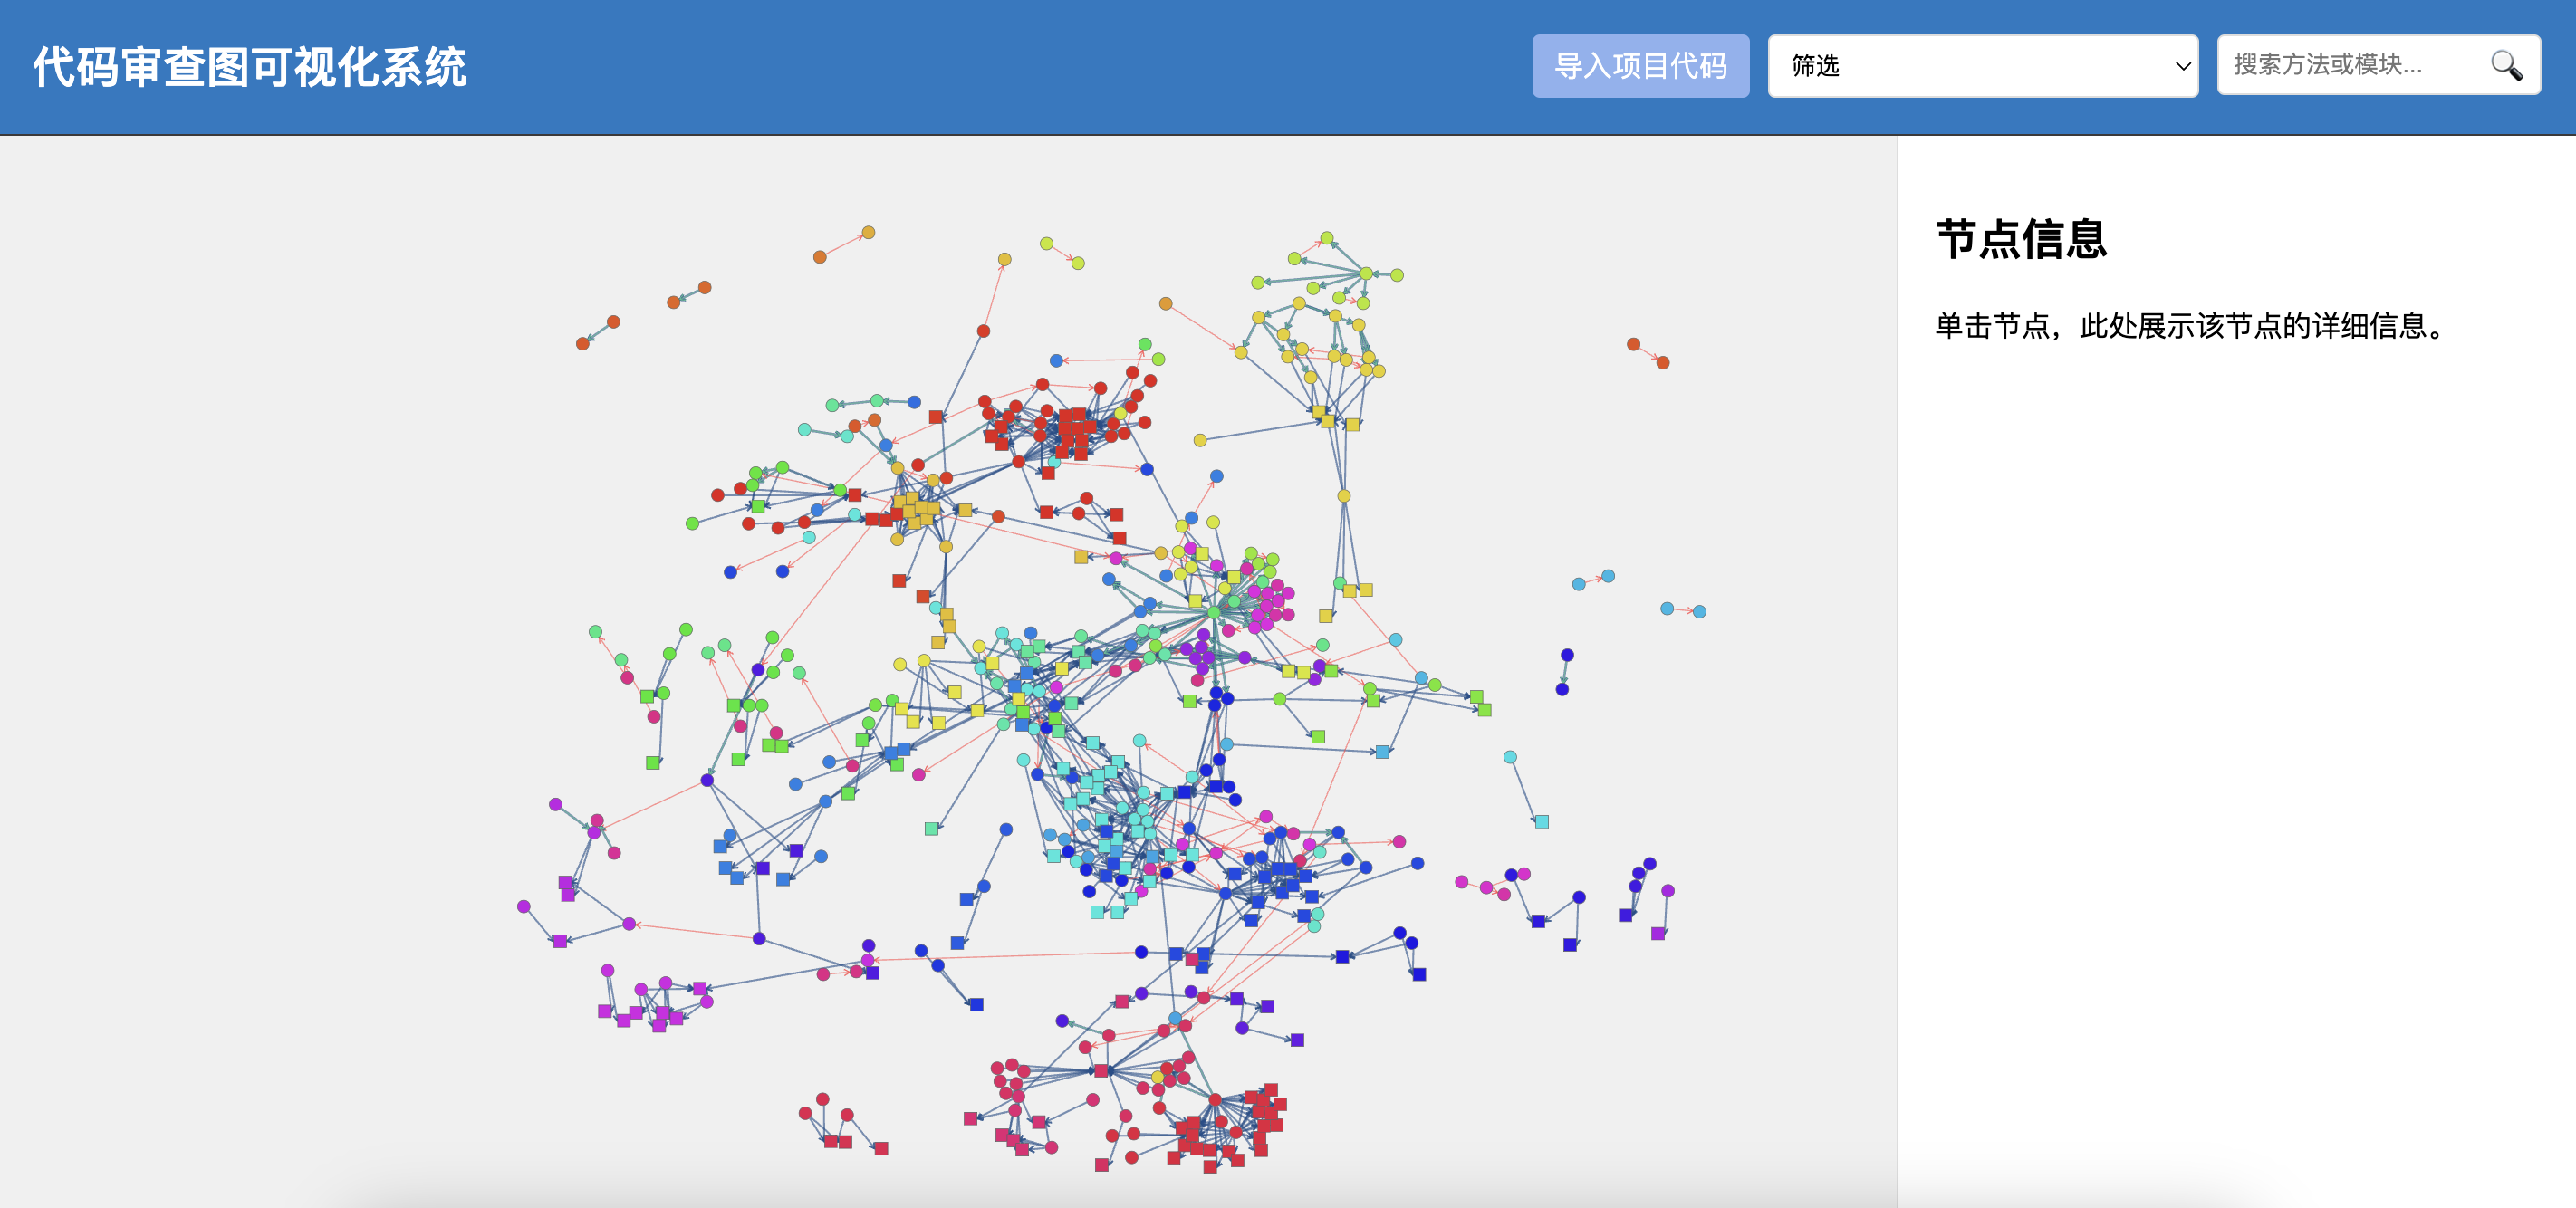
\includegraphics[width = 1.0\textwidth]{figures/开发1.jpg}
\caption{导入项目生成代码审查图}
\label{1_导入项目生成代码审查图}
\end{figure}

\noindent(2)对于开发任务所在的代码上下文,通过搜索方法名找到其在代码审查图中的位置,点击节点查看方法详细信息和质量度量情况,如图\ref{1_定位开发任务涉及的方法,查看质量信息}所示。

\begin{figure}[h]
\centering
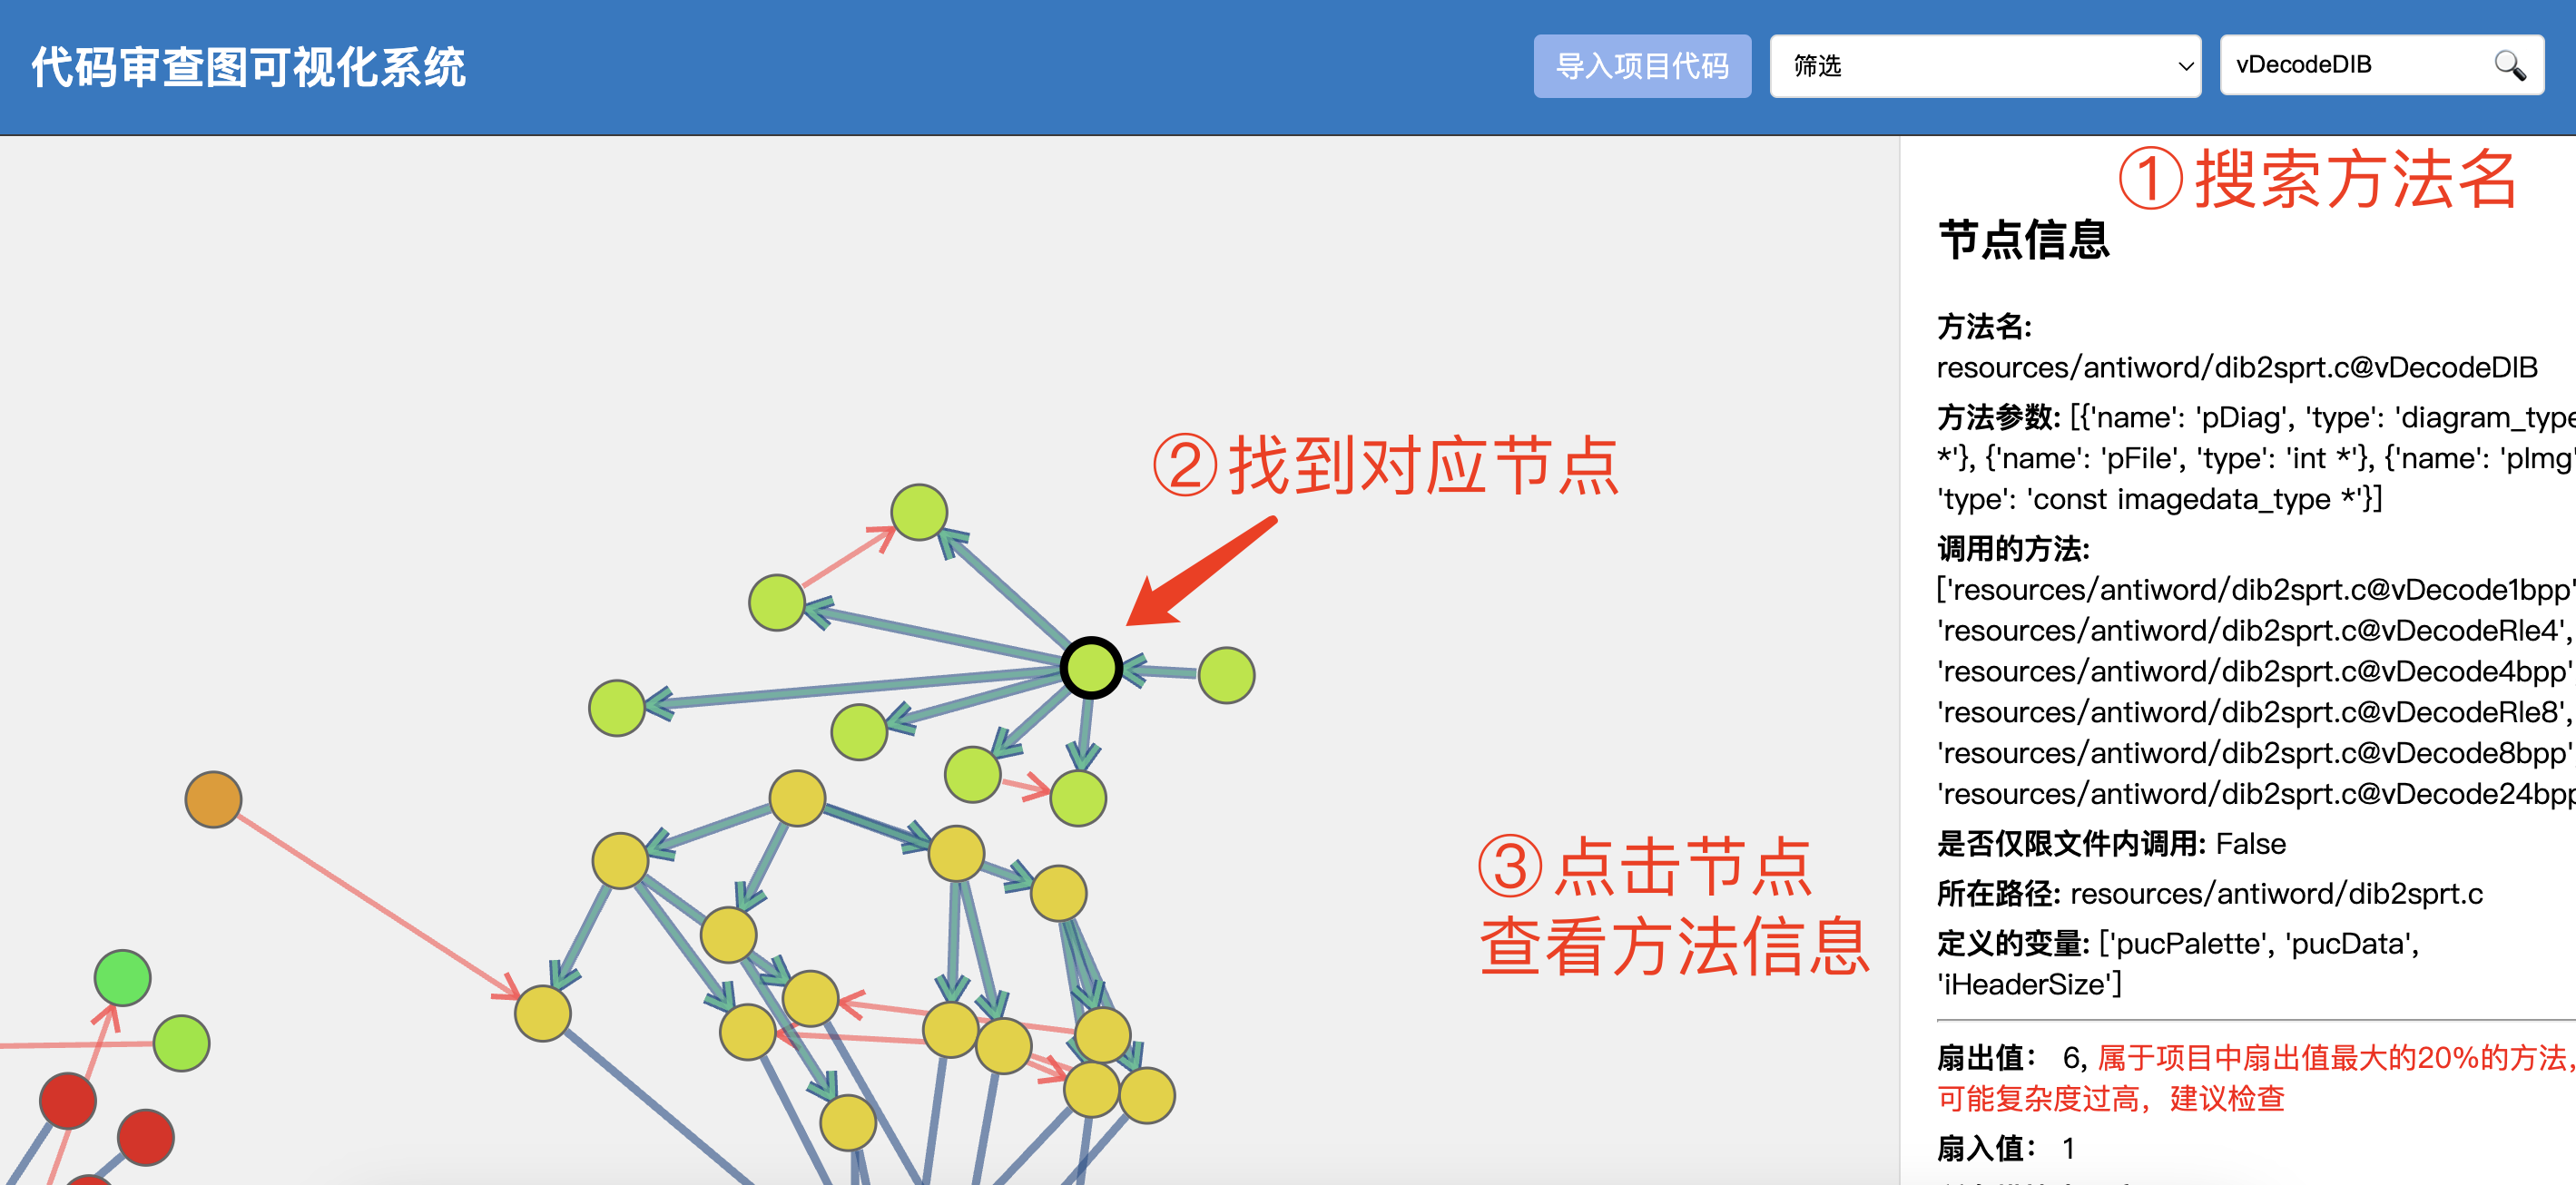
\includegraphics[width = 1.0\textwidth]{figures/开发2.jpg}
\caption{定位开发任务涉及的方法,查看质量信息}
\label{1_定位开发任务涉及的方法,查看质量信息}
\end{figure}

\noindent(3)根据代码审查图的边,则可以了解当前代码与其他部分的依赖关系、耦合关系和变更影响关系,如图\ref{1_查看方法对应边,按建议安全变更}所示。尤其是变更影响关系,可以帮助用户在进行变更时,提示变更方法所影响的范围,并根据给出的建议,帮助用户安全变更,解决了用户面对复杂软件难以理解、不敢变更、容易变更不完全的痛点。


\begin{figure}[h]
\centering
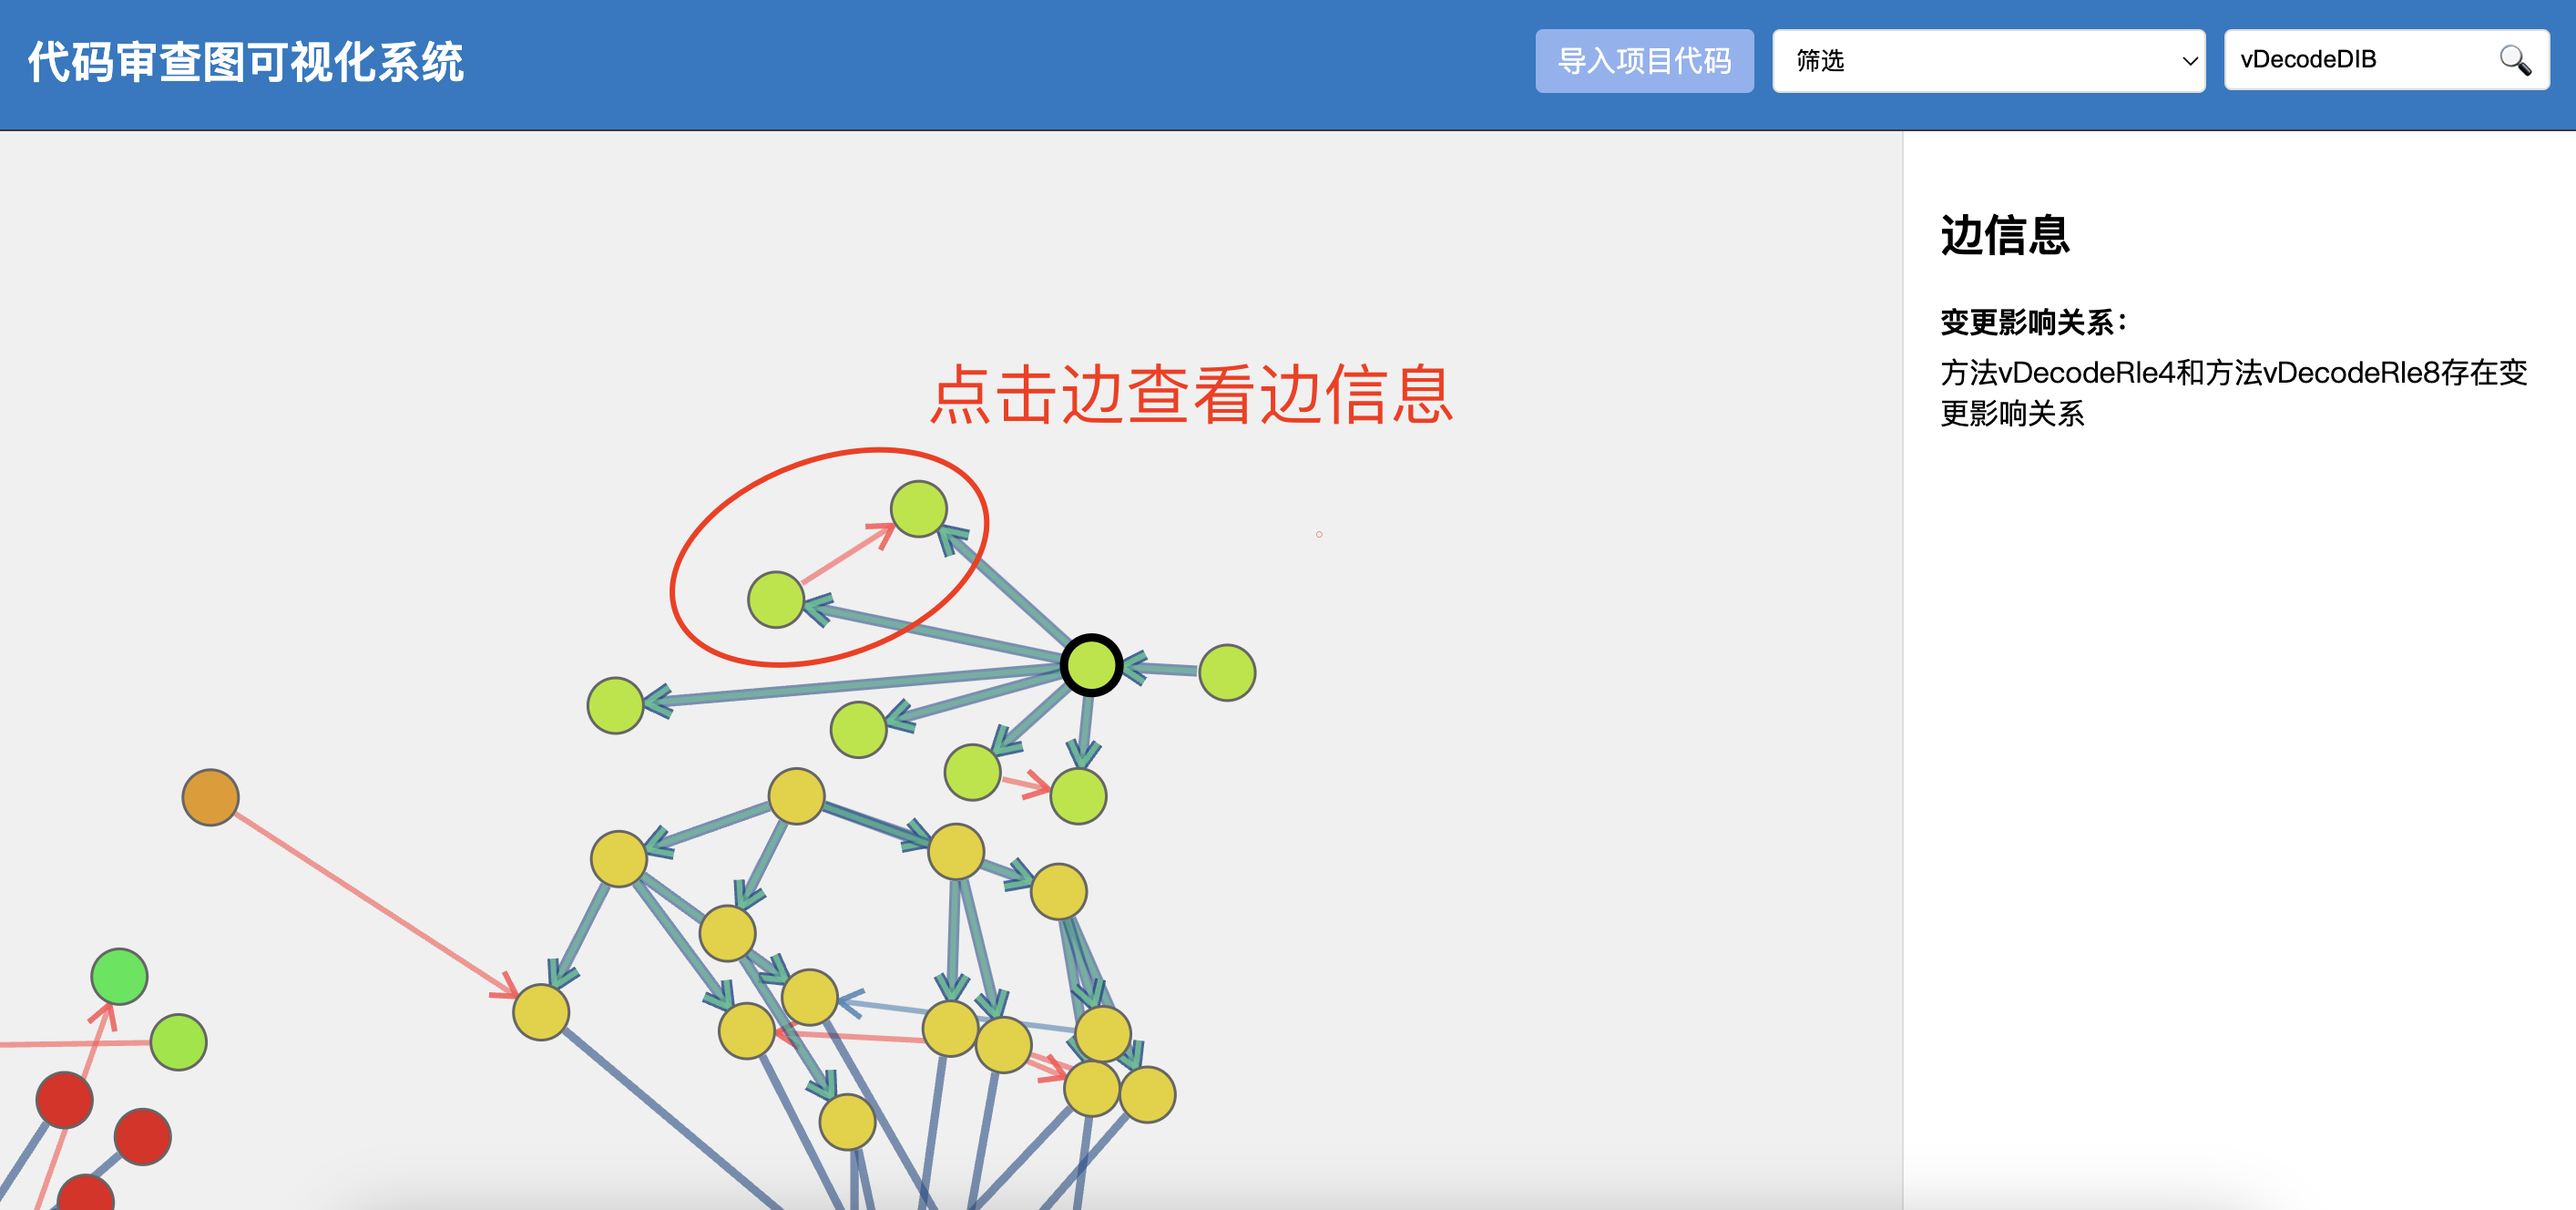
\includegraphics[width = 1.0\textwidth]{figures/开发3.jpg}
\caption{查看方法对应边,按建议安全变更}
\label{1_查看方法对应边,按建议安全变更}
\end{figure}

这里聚焦于 antiword 项目中的vDecodeDIB 方法的代码开发场景。若按照传统方法对该方法进行开发或分析,人工阅读代码需要涉及 300 多行代码的逻辑才能全面掌握方法的上下文。然而,通过代码审查图,开发者只需关注 8 个节点和 9 条边,即可快速获取关键信息。这种直观的可视化显著降低了代码理解的复杂度和成本。

\begin{figure}[h]
\centering
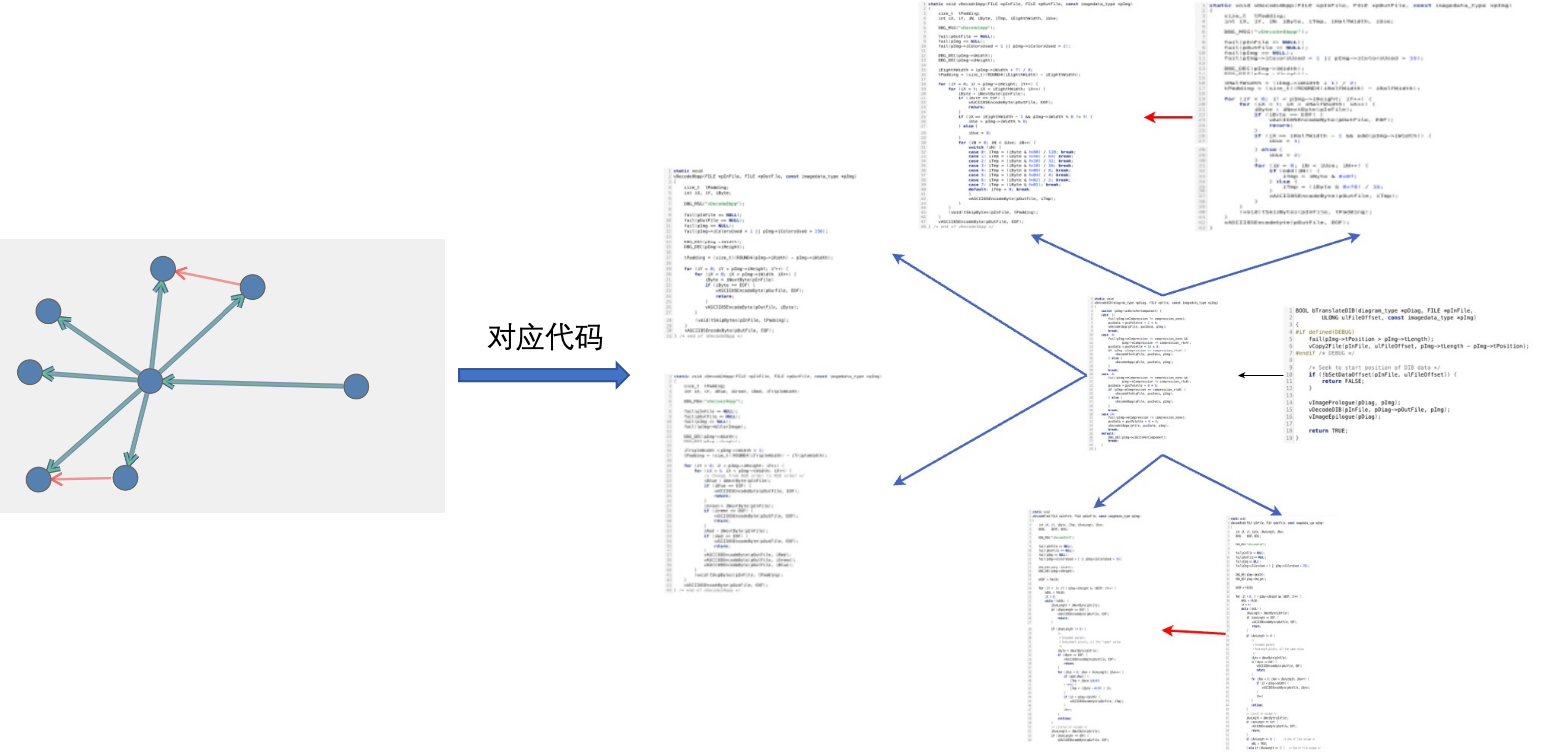
\includegraphics[width = 1\textwidth]{figures/3_助读示意.png}
\caption{vDecodeDIB方法上下文}
\end{figure}

尤其值得注意的是,该方法的上下文中包含了两个由于克隆代码导致的变更影响关系。这类关系通常隐匿于代码中,开发者仅靠手动查看代码很难准确发现并更改。代码审查图将这些隐藏的逻辑变更影响关系显式标出,使开发者在代码修改时能够快速识别潜在的影响范围,从而避免遗漏变更的风险。

\noindent \textbf{3.作为一种审查工具帮助审查者进行代码审查} 

当面对审查任务时,审查者可通过类似开发的过程,搜索代码审查图定位到当前提交所涉及的节点,通过图中的关系迅速了解代码上下文间的调用以及变更影响关系,通过系统的提示,对开发者的变更进行审查,检查其功能逻辑上是否安全变更,检查其变更操作给软件带来的质量影响是恶化还是优化,从而给出对应的审查结果。

\section{本章小结}

本章首先构建了一个代码质量度量模型,从五个维度对软件内部代码的相对质量展开评价。随后提出以代码审查图呈现软件结构和代码质量度量结果的可视化方式。随后,基于代码审查图开展代码质量分析,归纳出五种不良的图模式。借助这种方式,用户不仅能够更直观地把握代码结构,还能从宏观层面洞悉代码质量欠佳的缘由。通过实验验证了该代码质量度量模型能够切实有效地反映代码在重构过程中凸显的问题,进而证明了代码审查图在实际应用中的重要价值。最后,以案例分析的形式,展示了代码审查图在实际运用中的具体方法与显著优势。 
